% !TEX program = pdflatex
% !TEX enableSynctex = true
% !BIB program = bibtex

\documentclass[12pt]{article}

\usepackage{setspace}
\usepackage{amsmath}
\usepackage{amsfonts}
\usepackage{graphicx}
\usepackage{float}
\usepackage{dsfont}
\usepackage{natbib}
\addtolength{\oddsidemargin}{-.7in}
\addtolength{\evensidemargin}{-.7in}
\addtolength{\textwidth}{1.4in}
\usepackage{enumerate}
\onehalfspacing
\usepackage{geometry} % Required for customizing page layout
\usepackage{ragged2e}

\usepackage{caption}
\usepackage{booktabs}

\usepackage{hyperref}
\hypersetup{
	pdfstartview = FitH,
	pdfauthor = {...},
	pdftitle = {...},
	pdfkeywords = {...; ...; ...; ...},
	colorlinks = true,
	linkcolor = blue,
	urlcolor = blue,
	citecolor = blue,
	linktocpage=true
}

\DeclareMathOperator{\E}{\mathbb{E}}
\DeclareMathOperator*{\argmax}{arg\,max}
\DeclareMathOperator*{\argmin}{arg\,min}

\title{Liquidation Risk and Access to Cash Flow-Based Debt Finance}
\date{}

\begin{document}

\author{Barnabás Székely}
\date{\today}
\vspace{-1in}

\maketitle

\begin{abstract}
\noindent

This paper studies asset-based and cash flow-based lending in a heterogeneous firms model, where bankrupt firms may decide between liquidation or reorganization. The model highlights that creditors impose stricter terms on cash flow-based debt contracts if they believe that the borrower is likely to liquidate under financial distress. Since small and medium enterprises are often liquidated and lack pledgeable assets, they have limited access to both loan-types. This adds to the SME financing gap, yields misallocation of capital. Consequently, policy measures that facilitate the reorganization (such as the Small Business Reorganization Act) enhance allocative efficiency as they improve small firms' access to external finance. 

\bigskip{}
\bigskip{}
%\bigskip{}
%\bigskip{}
%\vspace{-0.5cm}

Keywords: Heterogeneous firms, Credit market frictions, Cash flow-based lending, SME financing gap
\medskip{}
% JEL Classification Code: E32, C22, E27.
\end{abstract}
\thispagestyle{empty}

\pagebreak{}


\section{Introduction \label{sec:introduction}} 
\textbf{Maybe, the best way to start is to follow the slides from the latest presentation.} Corporate credit market frictions are typically characterized as borrowing constraints defined the by value of pledgeable assets. Recent research has challenged this view based on more granular analyses of corporate credit contracts. These argue that the majority of corporate debt is backed by borrowers’ future cash flows rather than assets, which implies that credit frictions are better described as borrowing constraints defined by current earnings. These results led to several contributions focused on re-assessing credit market frictions in structural analyses. \vspace{3mm} \\
However, such studies typically adopt a `no equilibrium defaults' framework,\footnote{Dating back to Kiyotaki and Moore (1997).} where lenders impose borrowing limits to such that firms always meet their debt obligations. This gives rise to `hard constraints' to borrowing. Firms that borrow against assets are constrained by the value of their collateral, whereas those borrowing against cash flows are limited by current earnings. One shortcoming of this framework is its inability to account for variations of interest rates across firms - since debt contracts are always honored, every firm faces the same risk-free rate. This directed the focus of this literature to studying the effects of debt covenants,\footnote{These are legally binding agreements imposed by the creditor on the lender, that typically take the form of hard constraints implied by the no equilibrium defaults framework.} while credit spreads received considerably less attention.  \vspace*{3mm} \\
I fill this gap in the literature by studying the determinants of credit spreads for asset-based and cash flow-based debt. This requires a model framework where a certain proportion of firms choose to file for bankruptcy each period. Moreover, debt may be backed by assets, such that lenders' in-default payments are determined by their liquidation value, or by future cash flows, such that lenders' in-default payments reflect the going-concern value of the firm. Lenders set interest rates following their exposure to default and the probability of this event. Both of these increase with debt, causing interest rates to rise with borrowing. This yields `soft borrowing constraints', specific to firms' current state, credit demand and debt financing strategy, which allows me the structural analysis of credit spreads while considering heterogeneity in debt contracts. \vspace*{3mm} \\
\textbf{Here, mention the empirical analysis and find a segway to the importance of the liquidation probability} The structural model is supported by an empirical analysis of debt US debt contracts between 2010-2023. For both type of debt, I observe a negative relationship between credit spreads and the probability of liquidation, as well as assets. This finding contradicts the predictions of `hard constraints framework' as it suggests that size and profitability are important determinants of credit market frictions regardless of the type of borrowing. \vspace{3mm} \\
Bankrupt firms may undergo liquidation or reorganization (Chapter 7 and Chapter 11 in the US bankruptcy code). In the absence of collateral, the lender may retrieve only a fraction of the borrower's liquidation value. Hence, CF-based debt is backed mainly by the belief that the borrower would produce positive cash-flows even after experiencing financial distress. Choosing liquidation in bankruptcy terminates all future cash-flows. \textit{This turns the lending problem, into commitment issue.} \vspace{3mm} \\
Hence, high ex-ante probability of liquidation raises the credit spread of CF-based debt, by increasing lenders' exposure to default. Crucially, the proportion of liquidating firms decreases sharply with size. For instance, 56.6\% of firms with less than 100 million USD worth of total assets liquidate, but only 4.27\% of firms larger than this do so. I argue that in the case of CF-based debt, the value of assets serves as a proxy of liquidation probability rather than a direct determinant of in-default payments. \vspace*{3mm} \\ 
To study the impact of this trend, I consider endogenous liquidation decision in structural the model, similar to Corbae and D'Erasmo (2021). Firms in financial distress may  be liquidated, which entails exiting the market, or reorganized, which allows them to continue but incurs significant fixed costs.\footnote{These are generated by the time, legal and personnel expenses involving the renegotiation of debt \textit(cit).} This introduces economies of scale in reorganizations. Small firms are at a disadvantage under both type of debt contracts. Their access to CF-based debt is limited by high liquidation probabilities, while their access to asset based debt is limited by the amount of pledgeable assets. The model suggest that these compounding disadvantages are an important source of capital misallocation. However, bankruptcy framework that incentivise and facilitate small firm reorganization can mitigate this effect. \vspace*{3mm} \\
The paper is organized as follows. Section 2 reviews the related literature. Section 3 addresses the empirical analysis, beginning with a description of the data and the classification of debt contracts into asset-based and cash flow-based. It then presents descriptive statistics for debt contracts and firm characteristics. Lastly, it analyzes the empirical predictors of credit spreads and debt financing strategies. Section 4 introduces the structural model and section 5 discusses the results. Section 6 concludes.

\section{Literature \label{sec:literature}} 
Lian and Ma (2021) finds that majority of US corporate debt is backed by future cash flows rather than specific physical assets, which suggests that credit frictions are better described as earnings-based constraints. They support this finding by documenting the extensive use of earnings-based covenants in US corporate debt contracts. Similarly, Drechsel (2023) finds that three of the four most frequently used debt covenants limit debt based on current earnings rather than assets. \vspace{3mm} \\
These results led to the reevaluation credit frictions in macroeconomic models. Switching to earnings based constraints have been shown to have substantial impact on various model outcomes. Lian and Ma (2021) argues that this mitigates the financial acceleration driven by feedback of asset prices into credit constraints.\footnote{This mechanism was first highlighted by Bernanke, Gertler, and Gilchrist (1999).} Drechsel and Kim (2022) argues that firms subject to earnings based constraints under-borrow, while those facing asset based constraints over-borrow. Drechsel (2023) considers `investment shocks' that move the price of the capital countercyclically. He demonstrates that the effects of such shocks are heterogeneous depending on the borrowing constraint in place.  \vspace{3mm} \\
Earnings-based constraints have also been studied in relation to monetary policy, since unlike asset-based constraints, these directly interact with sticky prices. Greenwald (2019) points out interest coverage covenants, which limit borrowing in the ratio of interest payments to earnings introduce a direct channel of monetary policy transmission. Caglio, Darst and Kalemli-Ozcan (2021) studies the investment and credit channel of monetary policy when firms are backed by different type of collateral. They document that small and risky firms often rely on `going-concern value' collateral, which makes them more responsive to monetary policy shocks. \vspace{3mm} \\
The structural model proposed here adopts the heterogeneous firms framework established by Khan, Senga and Thomas (2013). This framework has been extended to study the decision to borrow against assets or cash flows. Öztürk (2023) highlights the volatility of earnings and pledgeability as important determinants of this decision. Gonzalez and Sy (2024) documents on Spanish data that reliance to CF-based borrowing (CF-based debt to total debt) is U-shaped across firms size, meaning that small and large firms borrow most against cash flows. On the other hand, empirical research such as Kermani and Ma (2020) highlight the importance of `asset specificity,' which describes how much value assets would lose under liquidation. \footnote{These papers are closely related to my research, since credit conditions and the debt financing strategy are jointly determined. Firms react to the credit conditions set by debt covenants and credit spreads by optimizing their debt financing strategy, which in turn affects the credit market frictions they eventually face.} \vspace{3mm} \\
Both Öztürk (2023) and Gonzalez and Sy (2024) adopt the `hard constraints' framework where firms choose between earnings-based or asset-based constraints based on which is less restrictive. In essence, this amounts to modelling heterogeneity in borrowing constraints. This approach does not allow for holding both types of debt simultaneously, which can be a significant limitation, since in the United States these borrowers represent a substantial share of the market. 
Conversely, I consider heterogeneity in debt contracts (differences in in-default payoffs) rather than borrowing constraints. This yields a more flexible framework that allows for firms that hold type of debt simultaneously. \vspace{3mm} \\
As mentioned above, I also consider in-equilibrium defaults and a liquidation decision similar to Corbae and D'Erasmo (2021), which implies lenders must account for the probability that the borrower would be liquidated under financial distress. However, they do not consider heterogeneity in debt contracts, meaning lenders and borrowers do not need to decide ex-ante whether the debt should be backed by assets or future cash flows. This yields more flexibility in collecting in-default payments, depending on the liquidation or reorganization decision of the firm.  \vspace{3mm} \\
Research into credit market frictions under asset-based and CF-based contracts typically focuses on the role of debt covenants, while credit spreads received considerably less attention. However, a closely related branch of empirical literature studies the role of different types of collateral in reducing credit spreads -  Cerqueiro, Ongena, Roszbach (2016), Luck and Santos (2020), Benmelech, Kumar and Rajan (2022). These studies must address endogeneity due to firms' self-selection into collateralized and uncollaterialized borrowers. They overcome this issue by using firm, bank, and time fixed effects, which yields plausible identification, but it restricts analyses to firms that borrowed both with and without collateral from the same lender within the same time period. Once its effect is adequately identified, collateral is to decrease credit spreads, but the strength of this effect varies across different types of collateral. \vspace{3mm} \\
Another related strand literature studies the role of unsecured debt in inducing investment (Biguri, 2020) or exacerbating credit cycles (Azariadis, Kaas and Wen, 2016). Moreover, Rampnini and Viswanathan (2022) studies firms' decision to borrow secured or unsecured. Note that categorizing debt as secured or unsecured is not analogous to differentiating asset-based and cash flow-based debt. The former relates to priority in bankruptcy, whereas the latter considers the economic determinants of lenders' in-default payoffs. Finally, I study the misallocation caused by the limited access to external finance. For extensive reviews of this the misallocation literature, see Restuccia and Rogerson (2012) and Hopenhayn (2014).

\section{Empirical analysis \label{sec:empirical analysis}}
This section presents the empirical analysis of the debt financing strategies, and liquidation decisions of US firms. I study a total of 113,774 debt contracts held by 6,925 non-financial corporations between 2010Q1 and 2023Q2. Debt-level data is provided by S\&P's Capital IQ and firm-level data is from Compustat North America. This yields and broad, but not representative sample of US non-financial corporations and their debt financing strategies. Moreover, I present evidence from Federal Judicial Center's Integrated Database (IDB), which contains a total of 160,367 Chapter 7 and Chapter 11 bankruptcy filings over the same period. \vspace{3mm} \\
Table 1. presents firm-level summary statistics for indicators of size, financial position, and borrowing conditions. Table 2. presents debt-level summary statistics, for contract value, maturity interest rates and spreads. 

\begin{table}[H] 
    \centering
    \resizebox{0.95\textwidth}{!}{%
    \begin{tabular}{lrrrrrr}
    \multicolumn{7}{l}{\textbf{Firm-Level Summary Statistics}} \\
    \hline
        & \textbf{Mean} & \textbf{p10} & \textbf{p25} & \textbf{Median} & \textbf{p75} & \textbf{p90} \vspace{1mm} \\
    Total Assets (millions USD) & 5235.16 & 11.39 & 73.11 & 582.60 & 2696.20 & 9567.60 \\
    Qtr. Revenue (millions USD) & 1073.75 & 0.18 & 8.77 & 109.62 & 551.79 & 1891.00 \\
    Employees (thousands) & 11.93 & 0.03 & 0.15 & 1.37 & 6.91 & 22.85 \\
    Firm Age (years) & 44.61 & 9 & 16 & 30 & 59 & 109 \\
    Cash to Assets (Liquidity) & 0.17 & 0.01 & 0.03 & 0.09 & 0.21 & 0.46 \\
    Debt to Assets (Leverage) & 0.30 & 0.03 & 0.12 & 0.27 & 0.43 & 0.61 \\
    Debt to Collateral & 0.51 & 0.11 &  0.26 &  0.52 & 0.75 & 0.89 \\ 
    Asset Pledgeability (\%) & 47.21 & 9.32 & 23.48 & 46.91 & 70.53 & 85.81 \\
    Total debt (millions USD) & 1817.35 & 1.06 & 8.33 & 132.69 & 960.90 & 3562.65 \\
    CF-share & 0.45 & 0.00 & 0.00 & 0.40 & 0.92 & 1.00 \\
    Average Maturity (years) & 6.7 & 1.4 & 4.0 & 6.1 & 8.6 & 12.2 \\
    Average Interest Rate (\%) & 4.9 & 0.3 & 2.7  & 4.6 & 6.8 & 9.2 \\
    Average Spread & 2.9  & 0 & 0.6 & 2.3 & 4.4 & 6.9 \\
    \hline
    \end{tabular}%
    }
    \caption{\small Summary Statistics - non-financial corporations between 2010Q1 and 2023Q2}
    \label{tab:sumstat}
\end{table}
\begin{table}[H]
    \centering
    \resizebox{0.95\textwidth}{!}{%
    \begin{tabular}{lrrrrrr}
    \multicolumn{7}{l}{\textbf{Debt-Level Summary Statistics}} \\
    \toprule
      	& \textbf{Mean} & \textbf{p10} & \textbf{p25} & \textbf{Median} & \textbf{p75} & \textbf{p90} \vspace{1mm}\\
    Contract Value (millions USD) & 334.53  & 0.16 & 2.24 & 48.24 & 396.00 & 859.22 \\ 
    Maturity (years) & 9.275 & 2.50 & 4.50 & 7.00 & 10.00 & 20.00 \\
    Interest Rate (\%) & 5.79 & 2.12 & 3.60 & 5.25 & 7.38 & 10.00 \\
    Credit Spread & 4.03  & 0.87 & 1.88 & 3.45 & 5.49 & 8.06  \\
	\bottomrule
    \end{tabular}%
    }
    \caption{\small Summary Statistics - debt contracts between 2010Q1 and 2023Q2}
    \label{tab:sumstat}
\end{table}

\subsection{Classification of Debt Contracts \label{sec:classification}}
Classification into asset based and CF-based debt is conceptually different from the notion of secured and unsecured debt.\footnote{Even though they may be strongly correlated. This leads Gonzalez and Sy (2024) to treat them as empirical equivalents. This approach is acceptable when blanket liens are rarely used  as is case for the Spanish corporate credit market.} Security establishes priority in bankruptcy, dictating who `queues first' to collect payments if the firm goes under. Conversely, the distinction between asset-based and cash flow-based debt refers to the economic determinants of lenders' in-default payoffs. When debt is backed by specific physical assets, lenders' in-default payoffs reflect the liquidation value of these items. In the case of CF-based debt, no specific physical asset serves as collateral meaning that in-default payoffs are chiefly determined by the future cash-flows of the borrower. \vspace{3mm} \\
The classification strategy adopted here follows the principles outlined by Lian and Ma (2021). Debt contracts that are not explicitly secured by specific physical assets are classified as cash flow-based debt. Hence, debentures and other unsecured debt contracts are counted towards this category. Bonds and notes are also considered cash flow-based debt, as they are typically unsecured or secured against future cash flows - through liens on substantially all assets or equity. The exceptions to this are mortgage bonds, which are backed by real estate, and thus fall under the category of asset-based debt. Similarly, capitalized leases are also classified asset-based. Finally, I consider debt contracts that are categorized as `term loans', `revolving credit' or `other borrowings' by Capital IQ. Depending on the specifics of the contract, these can be asset-based and cash flow-based debt as well. To remain conservative about the share of cash flow-based debt, I classify these instruments as asset-based, unless they are unsecured.  \vspace{3mm} \\
I find that $52.7\%$ of debt contracts can be classified cash flow-based. Since these are often large in terms of value, they collectively constitute 76.7\% of the total debt by volume - this aligns well with the aggregate results reported by Lian and Ma (2021).\footnote{Nevertheless, it should be noted that due to data limitations, my approach is likely to yield a cruder classification.} The share of CF-based debt remains relatively stable (fluctuating within the range of 71.8\% to 79.8\%). However, it declines significantly in the year 2019 and remains subdued until the end of the sample period - see figure \ref{chart:CFLshare} in the appendix. 

\subsection{Determinants of Credit Spreads \label{sec:credit spreads}} 
In this section, I study the firm-level determinants of credit spreads for asset-based and cash flow-based debt contracts. \textit{Here it is probably worth saying something like ...although the focus of this study is effects of liquidation probability studying other determinants of credit spreads is worthwhile since...} Existing literature typically focuses on the role of debt covenants in this context. These lend themselves for empirical analyses, as they impose similar `hard constraints' to borrowing as predicted by structural models (see Drechsel, 2022). However, such `hard constraints' are typically derived under the assumption of no in-equilibrium defaults. The model presented in section 4 produces a positive share of bankrupt firms in equilibrium. This generates endogenous variations in the cost of external finance, as individual borrowers face different interest rate schedules depending on their current state. This shifts the focus of the analysis to credit spreads. \vspace{3mm} \\
Credit spreads are calculated as the difference of the interest rate and the treasury rate at the corresponding maturity. To ensure that the observed credit spread reflects the original terms of the debt contract, I consider debt contracts and the corresponding firm characteristics only at the time of issuance. The regression analysis is carried on the sub-samples of asset-based and CF-based debt contracts as well as the entire sample. In each specification, period fixed effects are used to control for unobservable aggregate determinants of credit spreads. The results are summarized by table 3. \vspace{3mm} \\
Firms with higher EBITDA\footnote{For the estimation, I take the log-modulus transformation of the values of EBITDA.} and larger total assets benefit from lower credit spreads on both asset-based and cash flow-based debt contracts. This suggests size and profitability are important determinants of financial frictions no matter the form of borrowing. Somewhat puzzlingly, earnings appear to have less influence on the spread of CF-based debt contracts, which may be explained by the pervasive use of earnings-based covenants that are not considered in these regressions.  \vspace{3mm} \\
Asset pledgeability is defined as the proportion of collateralizable assets to total assets.\footnote{See precise variable definitions in section ... of the Appendix.} It is associated with lower interest rates for asset-based debt contracts, but has has no significant effect in the case of CF-based contracts. Since this indicator measures the extent to which assets can be used as collateral, it comes as no surprise that it only has a significant effect on asset-based debt. Higher leverage is associated with higher credit spreads across all specifications, but this effect is more pronounced for cash flow-based debt. This results is also as expected, since high leverage raises the probability of default as well as lenders' exposure. The logarithm of age has a significant, negative effect on credit spreads, suggesting that strong creditor-debtor relationships can help reduce the cost of external finance.  \vspace{3mm} \\
The coefficient estimates for number of employees are not consistent across specifications. This variable have a limited economic impact, even if it is statistically significant, which indicates that total assets is a sufficient measure of firms size. Credit spreads for asset-based debt are mostly not influenced by sector fixed effects (partly because pledgeability captures sector-level differences), but borrowing against cash flows is significantly more expensive for certain industries such as construction and retail trade. Consistent with the idea that lender perception is more important for cash flow-based debt, lower credit ratings are associated with a significant increase in credit spreads. For asset-based debt, however, credit spreads only react to credit rating categories that indicate a high risk of default.  \vspace{3mm} \\
Finally, `CF share' measures the extent to which a firm relies on cash flow-based debt as a fraction of total debt. Since firms tend to hold asset-based and cash flow-based debt simultaneously, this measure often falls between zero and one.\footnote{Of all firms, 35.7\% of only hold asset based debt, and 12.2\% solely depend on cash flow-based financing. The rest, 52.1\% of firms hold both type of firms hold both type of debt contracts at the same time.} This contradicts prior structural models, which only consider purely asset-based or CF-based borrowers. CF share is correlated negatively with spreads of cash flow-based debt and positively with spreads of asset-based debt, suggesting that firms self-select into these types of debt based on their relative costs. This result underlines that debt financing is jointly determined with the credit spreads firms eventually face. To give a complete account of firms' optimization, section ... in the appendix studies firm characteristics that influence the optimal share of CF-based debt total debt. 

\begin{table}[H]
    \centering
    \caption{Spread}
    \label{tab:spread_table_new}
    \resizebox{\textwidth}{!}{%
    \begin{tabular}{lcccccc}
    \toprule
    & \multicolumn{2}{c}{All contracts} & \multicolumn{2}{c}{CF contracts} & \multicolumn{2}{c}{AB contracts} \\
    \cmidrule(lr){2-3} \cmidrule(lr){4-5} \cmidrule(lr){6-7}
    \textbf{LHS}: Spread & Value & SE & Value & SE & Value & SE \\
    \midrule
    Log of EBITDA & -0.161*** & (0.0106) & -0.112*** & (0.0121) & -0.203*** & (0.0203) \\
    Log of Assets & -0.375*** & (0.0473) & -0.381*** & (0.0583) & -0.308*** & (0.0838) \\
    Pledgeability & -0.467*** & (0.0867) & -0.0297 & (0.108) & -0.990*** & (0.144) \\
    Leverage & 1.783*** & (0.103) & 2.278*** & (0.134) & 0.985*** & (0.168) \\
    Log of Age & -0.136*** & (0.0255) & -0.132*** & (0.0300) & -0.149*** & (0.0447) \\
    Log of Employees & -0.0118 & (0.0198) & -0.0974*** & (0.0252) & 0.0838*** & (0.0310) \\
    CF Share & 0.450*** & (0.0642) & -0.335*** & (0.112) & 0.748*** & (0.112) \vspace{3mm} \\

    \multicolumn{7}{l}{\textbf{Industries} - baseline: Agriculture and Fishing} \\
    Construction  & 0.739*** & (0.269) & 1.200*** & (0.461) & 0.275 & (0.375) \\
    Manufacturing  & 0.278 & (0.242) & 0.613 & (0.446) & 0.126 & (0.310) \\
    Mining & 0.847*** & (0.250) & 0.986** & (0.455) & 0.716** & (0.333) \\
    Retail Trade  & 0.677*** & (0.255) & 1.228*** & (0.455) & 0.0613 & (0.338) \\
    Services & 0.278 & (0.247) & 0.729 & (0.448) & -0.172 & (0.320) \\
    Public Utilities & 0.603** & (0.247) & 0.908** & (0.449) & 0.314 & (0.330) \\
    Wholesale Trade & 0.663** & (0.262) & 0.716 & (0.461) & 0.561 & (0.345) \vspace{3mm} \\
    \multicolumn{7}{l}{\textbf{Credit Ratings} - baseline: Rating: A} \\
    Rating: A+ & 0.163* & (0.0928) & 0.391*** & (0.0857) & -0.417 & (0.568) \\
    Rating: A- &  0.170** & (0.0765) & 0.197*** & (0.0653) & -0.0652 & (0.361) \\
    Rating: B+ & 0.723*** & (0.0713) & 0.726*** & (0.0653) & 0.157 & (0.325) \\
    Rating: B & 0.213*** & (0.0679) & 0.140** & (0.0583) & -0.0439 & (0.329) \\
    Rating: B- & 0.986*** & (0.0718) & 1.180*** & (0.0687) & 0.206 & (0.323) \\
    Rating: C  & 1.711*** & (0.0812) & 1.679*** & (0.0896) & 1.108*** & (0.326) \\
    Rating: D & 2.023*** & (0.140) & 2.434*** & (0.185) & 1.073*** & (0.362)  \\
    \midrule
    Period fixed effects & Yes & & Yes & & Yes & \\
    Observations & 17,668 & & 10,676 & & 6,992 & \\
    R-squared & 0.286 & & 0.403 & & 0.173 & \\
    \bottomrule
    \multicolumn{7}{c}{Robust standard errors in parentheses} \\
    \multicolumn{7}{c}{*** p$<$0.01, ** p$<$0.05, * p$<$0.1} \\
    \end{tabular}%
    }
\end{table}

\subsection{Liquidation Probability and Credit Spreads \label{sec:emp liqprob}} 
As argued in section ..., creditors may impose stricter terms on CF-based debt contracts if they believe the borrower is more likely to liquidate under financial distress. Although this `perceived risk of liquidation' is not directly observable, the empirical analysis provides indirect evidence that liquidation probability is in fact an important determinant of credit spreads.  \vspace{3mm} \\ 
Table 3 shows that the external finance premium decreases with total assets. However, in the case of CF-based debt the insignificant coefficient of pledgeability suggests that lenders do not do not value these assets as collateral. This raises the question: why do lenders value assets if not for seizing them in the event of bankruptcy? Figure ... documents that small firms often choose liquidation, whereas large firms typically reorganize. Hence, total assets can also be interpreted as a predictor of liquidation probability rather than a direct determinant of in-default payoffs. In the case of CF-based lending, he emphasis on total assets without regard of pledgeability suggests that creditors indeed take this into consideration when setting the terms of the debt contract. \vspace{3mm} \\ 
I test the robustness of these results in several alternative model specifications. Since, calculating credit spreads is subject to some uncertainty, the regressions in table 3 are repeated with interest rate as the dependent variable. In this case, debt maturity is also considered in the regression. Limiting the analysis to new issuances reduces the sample size. By using a weighted average of firm-level credit spreads as the outcome variable, I can examine the factors influencing external finance premia beyond the time of issuance. In this case, I consider three alternative samples: firms that borrow only against assets, only against cash flows and the set all firms. These regression results are presented in table ... and ... of the appendix. The central findings on this section remain largely unchanged across all alternative specifications. 
 
 \begin{figure}[H]  % [h] indicates placing the image here
    \centering  \label{chart:mixplot}
    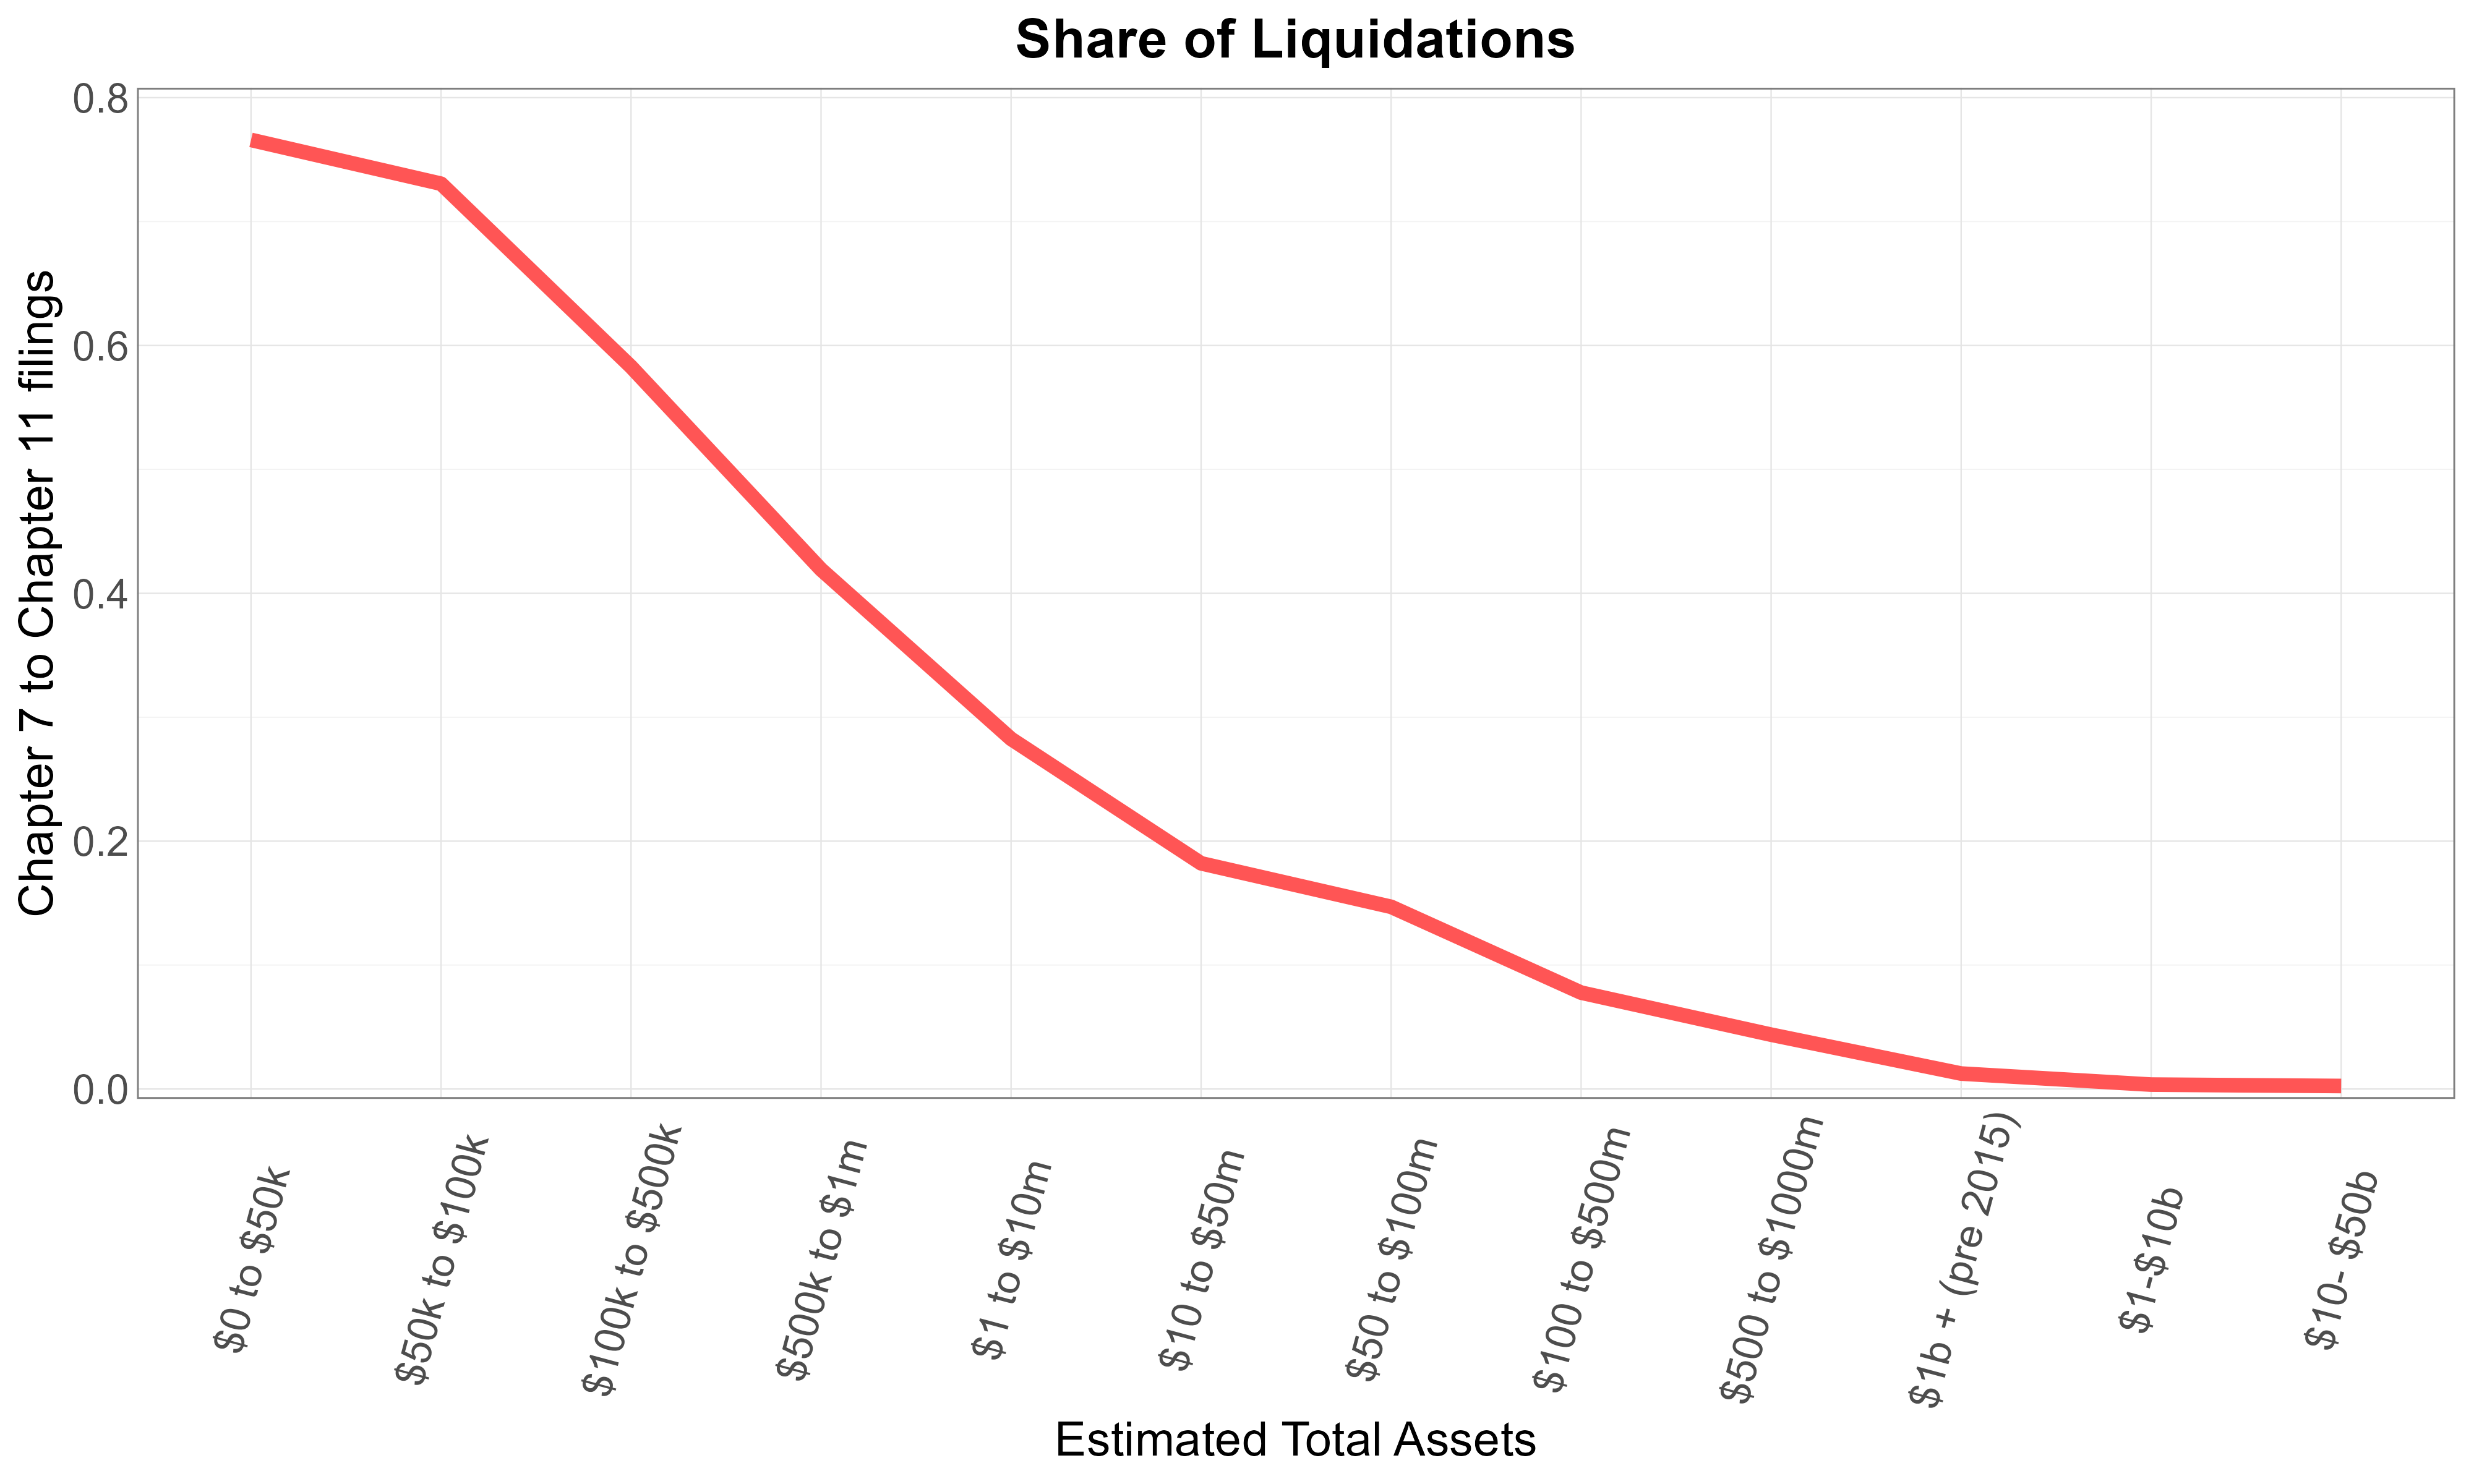
\includegraphics[width=1\textwidth]{C:/Users/szjud/OneDrive/Asztali gép/EBCs/CFL-git/Latex codes/Plots/liqprob2.png}
     \footnotesize \justifying Panel A. shows the all chapter 7 and 11 instances between 2010 and 2023. Panel B. shows the proportion of chapter 7 filings as a share to total bankruptcies. The figure shows that the probability of liquidation is decreases steeply with firm size. 
\end{figure}

\subsection{Limitations}
In the absence of natural experiments, empirical analyses are subject to considerable limitations. As discussed earlier, firms' endogenously adopt their debt financing strategy to credit conditions, which then affects the external finance premia they eventually face. Similarly, certain determinants of access to debt finance are difficult to observe. In this paper, I highlight the probability of liquidation, but other important factors such as assets specificity (Kermani and Ma, 2020) or the quality of accounting practices and court enforceability (Lian and Ma, 2021) may be similarly elusive. These shortcomings impede the identification of causal relationships between firm characteristics and credit spreads. The structural model discussed below makes up for some of these limitations. 


\section{Model outline} \label{sec:model}
In this section, I study asset-based and CF-based lending in a heterogenous firms model with in-equilibrium defaults and endogenous liquidation decisions. The model highlights the role of the ex-ante probability of liquidation, which has largely been overlooked in previous analyses. I find that liquidation risk raises the credit spread for CF-based debt. Since small firms are often liquidated in default, their access to CF-based debt is limited. Additionally, these firms have limited access to asset-based debt due to the lack of pledgeable assets. These compounding disadvantages lead to misallocation of capital which translates into a significant aggregate productivity loss. Along with liquidation risk, the model also captures the effects the other, more often discussed determinants of credit spreads such as leverage, size or productivity.\footnote{To keep the model parsimonious, I do not consider differences in asset pledgeability or asset specificity. This would be a straightforward extension to the model, but incorporating an additional state variable (describing firm-specific asset pledgeability) would make the computational burden unmanageable. Finally, I do not consider effects of firm age on credit conditions. To explore the effects of this determinant, one would have to consider a Bayesian learning mechanism as well as information asymmetries between creditors and lenders. This is beyond the scope of this paper.}

\subsection{Firms and production \label{sec:production}}
Heterogeneous firms produce a homogeneous consumption good, using labour $n$ and capital $k$. Firms are competitive, and face a decreasing returns to scale production technology:
\begin{equation} \label{eq:prodf}
y = \varepsilon k^{\alpha}n^{\nu}, \ \ \ \ \alpha,\nu \in (0,1),  \ \nu + \alpha \in (0,1)
\end{equation}  
where $\varepsilon$ is the idiosyncratic productivity state. In the interest of keeping the notation simple, I omit firm subscripts. \vspace{3mm} \\
Firms own capital and investments are financed partly by retained earnings and partly by borrowing from a competitive lender. A firm can be described by the predetermined capital stock $k \in \mathbf{K} \subset \mathbf{R^{+}}$, debt $b \in \mathbf{B} \subset \mathbf{R}$ and current productivity $\varepsilon \subset \mathbf{R^+}$. Idiosyncratic productivity is a Markov chain on the finite set $\varepsilon \in \mathbf{E} \equiv \{ \varepsilon_1,...,\varepsilon_{N_{\varepsilon}} \}$ such that $ g_{ij} \equiv \Pr(\varepsilon'= \varepsilon_j|\varepsilon = \varepsilon_i) \geq 0$ and $\sum_{j=1}^{N_{\varepsilon}} g_{ij} = 1$ for each $i$. Moreover, it is stochastically monotone such that for any fixed $x$, $\Pr(\varepsilon' \leq x | \varepsilon = \varepsilon_i)$ is decreasing in $\varepsilon_i$. \vspace{3mm} \\
Production occurs before the realization of exit and entry decisions take effect, and optimal labor demand is independent of current debt. Therefore, at the beginning of the period every firm of state vector $(k,\varepsilon)$ faces the same static optimization with respect to labour: 
$$ \pi(k,\varepsilon) = \max_{n} \ \  \varepsilon k^{\alpha}n^{\nu} - wn - c$$
where $c$ is a fixed cost of participating in production, $w$ is the wage and the price of the consumption good is flexible and normalized to $1$. Optimization yields the policy function for labour demand, $n(\varepsilon,k)$ and optimal production $y(\varepsilon,k)$: 
\begin{equation} \label{eq:opt_emp_prod}
n(k,\varepsilon) = \left( \dfrac{ \nu \varepsilon k^\alpha}{w} \right)^{\frac{1}{1-\nu}} \hspace{15mm}
y(k,\varepsilon) = \varepsilon k^{\alpha} \left( \dfrac{\nu \varepsilon k^\alpha}{w} \right)^{\frac{\nu}{1-\nu}}.
\end{equation}  
Firm profit function can be reformulated as: 
\begin{equation} \label{eq:profit}
\pi(k,\varepsilon) = y(k,\varepsilon) - wn(k,\varepsilon) - c = (1-\nu) y(k,\varepsilon) - c.
\end{equation} 
Firms own capital and make idiosyncratic investment decisions. Capital accumulation follows: 
\begin{equation} \label{eq:capital}
k' = (1-\delta)k + i
\end{equation} 
where $\delta$ is the depreciation rate and $i$ is investment. Finally, I describe firms' financial position by the cash on hand variable:
\begin{equation} \label{eq:cash on hand}
    x = \pi(k,\varepsilon) + (1-\delta)k - b.
\end{equation}
The distribution of firms can be summarized using the probability measure $\mu$ defined on the Borel algebra $A$, generated by the open subsets of the product spaces $ \mathbf{A} = \mathbf{K} \times \mathbf{B} \times \mathbf{E} $.

\subsection{Firm Values and the Default Decision } \label{sec:defaults}
Production takes place at the beginning of the period. Firms set their labour demand given $(k,\varepsilon)$, profits are realized and capital depreciates. Then, incumbents may decide to exit, default or continue production to the next period. This decision is governed by: 
\begin{equation} \label{eq:default decision}
    V(k,b,\varepsilon) = \max \{ V_{exit}(k,b,\varepsilon), \ V_{def}(k,b,\varepsilon), \ V_{cont}(k,b,\varepsilon) \}.
\end{equation}
Firms may decide to exit after settling their debt obligations, which allows them to retain the value of the depreciated capital stock net of debt service. Since this decision takes effect only after production, this amounts retaining the cash on hand
\begin{equation}
    V_{exit}(k, b, \varepsilon) = \pi(k,\varepsilon) + (1-\delta)k - b  = x.
\end{equation}
Default can be resolved by liquidation or reorganization. Under liquidation, the firm exits and \textit{all} of its undepreciated capital stock resold for $\phi_l(1-\delta)k$, where $\phi_l \in (0,1)$ indicates that corporate assets are often highly specialized and illiquid, which reduces their resale value. The lender cannot seize more than the value of the debt, hence the firm-value associated with liquidation is,
\begin{equation}
    V_{l}(k, b) = \max \{ 0, \ \phi_l(1-\delta)k - b  \}.
\end{equation}
Under reorganization, the firm pays a lump-sum $\Pi_{r}(k, b, \varepsilon)$ to the lender, allowing it to continue into the next period - this is discussed in detail in the following section. Moreover, reorganization incurs a fixed cost $\zeta_r$ which is borne entirely by the borrower.\footnote{The incidence of the fixed cost has a minimal effect credit market frictions. Lenders' expenses directly raise the external finance premium, whereas borrowers' costs limit access to external finance indirectly by raising liquidation risk.} This fixed cost introduces economies of scale into the reorganization process, hence it crucial in replicating the decreasing liquidation probability in the function of firm size - I discuss the sources of these costs in section \ref{sec:fixed costs} of the appendix. Taking stock, the value that the firm associates with reorganization is: 
\begin{equation}
    V_{r}(k, b, \varepsilon) = V_{cont}(k,b,\varepsilon) - \min\{b, \ \Pi_{r}(k, b, \varepsilon)\} - \zeta_r.
\end{equation}
Bankrupt firms may choose reorganization or liquidation such that the value of default is:
\begin{equation} \label{eq:liq or reorg}
    V_{def}(k, b, \varepsilon) = \max \{ V_{l}(k, b), \ V_{r}(k, b, \varepsilon)  \}.
\end{equation}
This formulation assumes that lenders' payoffs are not considered at the liquidation decision. This reflects the consideration that individual lenders often have a limited influence over the default resolution process - see in section \ref{sec:key principles} of the appendix. It also is worth noting that the model generates `voluntary' and `involuntary' defaults as well. Firms may decide to default if $V_{def}$ yields the highest value, as described in equation \ref{eq:default decision}. However, firms may also fail to reach a debt agreement that allows them to fulfill their debt obligations and pay non-negative dividends at the same time. In this case, they are forced tho choose between liquidation or reorganization, as described in equation \ref{eq:liq or reorg}.\footnote{Voluntary defaults can be found in Corbae and D'Erasmo (2021) and involuntary defaults in Khan and Thomas (2016).}  \vspace{3mm} \\
Firms that decide to continue may access external finance in the form of one-period debt contracts. For every unit of debt to be repaid in the next period, they receive $q$ units of output that may be allocated towards investment or distributed as dividends. Moreover, it is possible to borrow against physical assets or future cash flows. As discussed in the following section, these debt contracts differ only in the pay-offs they provide to lenders in case of default. In every other respect, the two loan-types are perfect substitutes, hence the total debt of held by the firm can be described as $b = b^C+b^A$. Analogously to the empirical analysis, I define CFL reliance as: 
\begin{equation}
    \tau = b^C/(b^C+b^A).
\end{equation}
Continuing firms choose future capital stock $k'$, total future debt $b'$ and debt financing strategy $\tau'$ to maximize the discounted sum of dividends, $d$ 
\begin{equation} \label{eq:dividends}
d = x - k' +  q(k',b',\varepsilon, \tau')b'.
\end{equation} 
The lending schedule faced by individual firms depends on current productivity and future values of capital and debt. These are free of adjustment costs, therefore they can be chosen independently from current stocks. Hence, for continuing firms, cash on hand and current productivity $(x, \varepsilon)$ are sufficient to describe the current state comprehensively.\footnote{This formulation reduces the computational burden of the model.} Using the cash on hand variable, the value of continuation can be described as,
\begin{equation} \label{eq:V_cont}
    V_{cont}(x,\varepsilon) = \max_{k',b', \tau'} \left(x - k' +  q(k',b',\varepsilon, \tau')b' + q_f \E_{\varepsilon'|\varepsilon} V(k',b', \varepsilon') \right)
\end{equation}
subject to: 
\begin{equation} \label{eq:budget}
x' = \pi(k',\varepsilon')+(1-\delta)k'-b' \hspace{5mm} \text{and} \hspace{5mm} d \geq 0
\end{equation} 
where $q_f$ is the firms' discount factor. \vspace{3mm} \\
I define the following indicator functions: $\chi_{r} = 1$ if the firm chooses reorganization, $\chi_l = 1$ if it chooses liquidation, and $\chi_{ex} = 1$ if it exits after fulfilling its debt obligations. To simplify notation, I summarize the collection of decision variables introduced above as $a = (k, b, \tau) $. In the next section, I discuss financial intermediation, which allows me to describe how the inverse gross interest rate $q(a',\varepsilon)$ depends on these decision variables and the current productivity.
\subsection{Financial Intermediation}  \label{sec: Financial Intermediation}
\subsubsection{The lender's problem}    \label{sec: The lender's problem}
The opportunity cost of lending to corporations is determined by the risk-free bond yield $q_0$. However, since corporate lending is subject to default risk, the competitive lender must charge a premium to break even. When setting $q(a',\varepsilon)$ the lender must consider the expected payoff under 3 distinct scenarios: \textit{a)} orderly repayment; \textit{b)} the firm defaults and is liquidated \textit{c)} the firm defaults and is reorganized.\footnote{Note that the lender cannot retrieve more than the initial value of the debt, as described by the minimum function in equation \ref{eq:q}.}  It follows from the zero-profit condition that the debt schedule offered to firms is, 
\begin{equation} \label{eq:q}
    \begin{split}
        & q(a', \varepsilon)b' = q_0 \left[ \left(1-P_D(a', \varepsilon)\right)b' + \right. \\
        & \qquad P_D(a', \varepsilon) \gamma(a', \varepsilon) \min \{b', \ \Pi_{l}(a')\} + \\ 
        & \qquad \left. P_D(a', \varepsilon) (1-\gamma(a', \varepsilon))\min \{b', \ E_{\varepsilon' | \varepsilon} [ \Pi_{r}(a', \varepsilon') |\chi_r = 1 ] \} \right]
    \end{split}
\end{equation}
where 
\begin{itemize}\setlength\itemsep{0em} 
    \item $\Pi_{l}(a')$ is the expected payoff if the firms undergoes liquidation,
    \item $\Pi_{r}(a', \varepsilon)$ is the expected payoff if the firms undergoes reorganization,
    \item $P_D(a', \varepsilon)$ is the endogenous probability of default,
    \item $\gamma(a', \varepsilon)$ is the probability of liquidation under financial distress. 
\end{itemize} 
In the following, I discuss the determinants of these values, which leads to the complete description of the debt schedule $q(a', \varepsilon)$.
 
\subsubsection{Lenders' Expected Payoffs}   \label{sec:Default Resolution}
This section describes lenders' expected, in-default pay-offs when debt is backed by physical assets or by future cash flows. These pay-offs are central to the analysis, as they shape the debt schedule $q(a', \varepsilon)$, that firms must consider in choosing debt financing strategy. In setting these expectations, the lender must consider that its exposure to default depends on borrowers' potential decision between liquidation and reorganization under financial distress. Hence, the lender calculates how much of the original debt can be recovered under four distinct cases \textit{1)} recovery of AB debt under liquidation, \textit{2)} recovery of CF debt under reorganization, \textit{3)} recovery of AB debt under reorganization, \textit{4)} recovery of CF debt under liquidation. \vspace{3mm} \\
When debt is backed by physical assets, the lender expects to retrieve in-default payments through liquidation. The absence of such securities in case of cash flow-based contracts reflects creditors' expectation that the firm would generate positive cash flows even after experiencing financial distress. This is possible only if the borrower is reorganized. Hence, in cases \#1 and \#2 the default resolution is `consistent' with the terms of the debt contract. These values easy to set based on prior literature. On the other hand, reorganization prevents the liquidation of physical assets (case \#3) and reorganization terminates all future cash flows (case \#4). Setting these values requires more thought. \vspace{3mm} \\
Take asset-based debt first. The main advantage of these debt contracts is that they provide a quick and cost-effective way to recover in-default payments by liquidating borrowers’ assets. Hence, in case of liquidation, the lender can extract the entire re-sale value of capital (case \#1). This case corresponds to the traditional approach to modelling financial frictions, which yields asset-based borrowing constraints. When the borrower undergoes reorganization (case \#3),  secured lenders are protected by the ‘best interest of creditor’ test.\footnote{The EU Directive refers this principle as ‘best-interest-of-creditors’ test in OJ L 172/27, art. 49; whereas the US bankruptcy code establishes this principle in 
 - see section \ref{sec:A1} in the appendix} This states that creditors cannot be worse off under the reorganization plan than they would be under of liquidation. Therefore, I assume that after asset-backed debt contracts, the lender expects to extract the full liquidation value, $\phi_l(1-\delta)k$ irrespective of the bankruptcy resolution. \vspace{3mm} \\
When debt is backed by future cash-flows the lender expects in-default payoffs from the reorganization of the borrower (case \#2). In this case, the lender can claim a fraction of the continuation value such that its payoff is $\phi_c V_{cont}(x,\varepsilon)$.\footnote{This is only a stylized description of the reorganization process. In practice, this often entails negotiations between the borrower and multiple creditors with potentially conflicting interests, under the supervision of courts. Moreover, the negotiating parties' bargaining power may depend on the specific terms outlined in the debt contract. I do not attempt to capture all this complexity in the model, as the focus on giving a precise account on lenders' in-default payoffs.} For an analogous description of lenders in-default payoffs, see Drechsel (2023) - he demonstrates that with no equilibrium defaults, this yields earnings based borrowing constraints. If this payoff exceeds the liquidation value of assets the lender may be able to offer more lenient credit terms. However, if the borrower is liquidated under financial distress, there are no future cash-flows to be claimed (case \#4). In this case, since the debt not backed by physical collateral, the lender can recover only a fraction $\kappa \in (0,1)$ of the liquidation value $ \phi_l(1-\delta)k$. \vspace{3mm} \\
Table \ref{tab:lender payoffs} summarizes the lender's payoffs for each debt contract and default resolution pair. This summarizes the central trade-off in the model. When debt is asset based the lender may expect to retrieve the liquidation value of the firm, irrespective of the default resolution. In contrast, when debt is CF-based the lender expects to retrieve a share of the continuation value under reorganization, but risks loosing out if liquidation occurs.

\begin{table}[h!]
    \centering
    \begin{tabular}{l|cc}
        & Liquidation  & Reorganization \\  
       \midrule
      Asset based debt & $ \phi_l (1-\delta) k$  &  $ \phi_l (1-\delta) k$ \\
      CF based debt & $ \kappa \phi_l (1-\delta) k $ & $ \phi_c V(x,\varepsilon)$ \\ 
     \bottomrule
     \end{tabular}
    \caption{\small The lender's payoffs under each default resolution, debt contract pair gross of fixed costs.} 
    \label{tab:lender payoffs}
\end{table}
\noindent It is now possible to outline the lender's expected payoff depending on the liquidation decision and the debt financing strategy adopted prior to bankruptcy. Recall that the share of CF-debt to total debt is defined by $\tau \in (0,1)$. Hence, the lender's payoff under liquidation (or reorganization) is a linear combination of the payoffs from asset-backed debt (with weight $\tau$) and CF-debt (with weight $1-\tau$). \vspace{3mm} \\
First, consider debt-recovery under liquidation. The liquidation value of the firm is: $\phi_l (1-\delta) k$. However, the lender can only retrieve this value for the debt that is backed by physical assets, which is $1-\tau$ share of the total debt. After the remaining $\tau$ share, which corresponds to CF-based debt, the lender can seize only $\kappa$ fraction of original liquidation value - see top-left and bottom-left of table \ref{tab:lender payoffs}. Taking stock, the if the borrower is liquidated the lender receives:\footnote{Note that this value might be smaller than what is taken from the firm in case of liquidation. For the sake of simplicity, I assume that the difference of the two is a welfare loss of the liquidation process.}  
\begin{equation} \label{eq:P_liq} 
   \Pi_{l}(a) = (1-\tau) \phi_l (1-\delta) k +\tau \kappa \phi_l  (1-\delta) k. 
\end{equation}
When the firm undergoes reorganization the lender can claim a fraction of future cash flows after CF-based debt. Moreover, in accordance with the `best interest of creditor test' the lender expects to retrieve a payment that is equal to the liquidation value of the collateral after asset-based debt - see bottom-right and top-right of table \ref{tab:lender payoffs}. Taking stock, when the borrower undergoes reorganization, the lender receives
\begin{equation}  \label{eq:P_reorg}
   \Pi_{r}(a,\tau) = (1-\tau) \phi_l (1-\delta) k +\tau \phi_c V_{cont} (x, \varepsilon).
\end{equation}
The borrower pays this value as a lump-sum to the lender. This stylized description of the reorganization process aims to capture the fact that in this case the lender's payoffs depends on the continuation value of the firm.  In practice, the means of extracting the continuation value may depend on the debt contract that is in place. When the debt is secured against the entire corporate entity, the lender may gain access to borrower's cash flows directly. When the debt is unsecured, higher continuation value of the firm allows the lender to negotiate better terms during reorganization. For a precise description of this mechanism see Corbae and D'Erasmo (2021). \vspace{3mm} \\
Finally, the probability default and liquidation can be defined using the indicator functions introduced in section \ref{sec:defaults}: 
\begin{equation} \label{eq:default probability}
    P_D(a',\varepsilon) = \E_{\varepsilon'|\varepsilon}[\chi_l(a',\varepsilon') + \chi_r(a',\varepsilon')],
\end{equation}
and
\begin{equation} \label{eq:liquidation probability}
    \gamma(a',\varepsilon) = \E_{\varepsilon' |\varepsilon}[\chi_l(a',\varepsilon')].
\end{equation}
Bringing default and liquidation probability (equation \ref{eq:default probability} and \ref{eq:liquidation probability}) and expected payoff under liquidation and reorganization (equation \ref{eq:P_liq} and \ref{eq:P_reorg} respectively) to the zero profit condition described in equation \ref{eq:q} yields a complete description of the debt schedule $q(a', \varepsilon)$ offered to firms. Firms choose the debt financing strategy that maximizes the continuation value as described in equation \ref{eq:V_cont} - \ref{eq:budget}.

\subsection{Firm dynamics}
Firm exits are balanced by a mass $M$ of potential entrants. These are endowed with zero starting cash on hand, reflecting that startups are typically asset-poor. Entrants' starting productivity is drawn from the stationary distribution of the Markov chain that defines idiosyncratic productivity - denoted by $\Phi(\varepsilon)$. Entrants do not produce in the first period, and have the option to exit after drawing a productivity value, if their continuation value is smaller than zero. Since potential entrants do not have prior debt obligations, they only need to solve \ref{eq:V_cont} - \ref{eq:budget}. If $V_{cont}(0,\varepsilon)$ is smaller than zero, they exit immediately, without ever participating in production. \vspace{3mm} \\
Let $\mu_0$ be the measure of the mass of firms at the beginning of the period. Using the indicator variables defined in \ref{sec:defaults}, the measure of firms at the end of the period can be defined as: $\mu = (1 - \chi_l - \chi_{ex}) \mu_0  + (1 - \chi_{ex}) M d \Phi(\varepsilon) $. The evolution of firm distribution then satisfies:
\begin{equation} \label{eq_firmdim} 
    \mu_{0}'(A) = \int \mathbf{I}_{(k', b', \varepsilon') \in A} g(\varepsilon'|\varepsilon) \ d \mu (k,b,\varepsilon)
\end{equation}
for all Borel sets $A \subset  \mathbf{K} \times \mathbf{B} \times \mathbf{E} $ and where $g(\varepsilon'|\varepsilon)$ is the transition probability matrix idiosyncratic productivity. Finally, I summarize the dynamics of firm distribution at the beginning of the period by the mapping $ \mu'_0 =\Gamma(\mu_0)$.

\subsection{Households}\label{sec:hh}
There is a unit measure of identical households that choose a stream of consumption $C$ and one-period, noncontingent bonds $B$ to maximize expected discounted utility. Households take firm measure $\mu_0$ as given. Their problem can be defined recursively as: 
\begin{equation} \label{eq:U_max}
V_h(B, \mu_0) = \max_{C,B'} U(C) + \beta V_h(B',\mu_0')
\end{equation}  
subject to: 
\begin{equation} \label{eq:const_hh}
C + B + \leq w N^s + q_0 B' + T
\end{equation} 
where $N^s$ is the inelastic labour supply and $\beta$ is the households' discount factor. \vspace{3mm} \\
Households share the expenses and revenues from the production sector. On the revenue side, they receive dividends from continuing firms and the net wealth from exiting firms. On the expense side, they are responsible for financing the reorganization of firms. These are collected into the lump-sum transfer $T$,
\begin{equation} \label{eq:T}
    \begin{split}
        & T = \int (1 - \chi_l - \chi_{ex}) \left( x - k'(k,b,\varepsilon) + qb'(k,b,\varepsilon) \right) d \mu_0(k,b,\varepsilon) \\
        & \qquad + \int \chi_{ex} \ x \ d \mu_0(k,b,\varepsilon) - \int \chi_{r} \ \Pi_r(k,b, \varepsilon) \ d \mu_0(k,b,\varepsilon)
    \end{split}
\end{equation}
Since firms are owned by households, future dividend payments are discounted using the household’s discount factor $\beta = q_f$. This implies that firm values represent marginal contributions to the household's utility.

\subsection{Stationary equilibrium}\label{sec:eq}
The stationary competitive equilibrium is described by the set of functions
$$(\mu_0, \mu, w, V, V_{cont}, V_{def},  V_{exit}, V_r, V_r, \chi_l, \chi_l, \chi_{ex}, n,k,b,d,\tau,q, C, B)$$
such that: 
\begin{enumerate}[(i)]
\item households solve utility maximization: $V_h$ solves \ref{eq:U_max}-\ref{eq:const_hh} and the associated policy functions are $(C, B)$;
\item the lender solves \ref{eq:q} such that $q(a',\varepsilon)$ yields zero profits in expectation on each debt contract;
\item firms solve value maximization: $V$ solves \ref{eq:default decision}, $V_{def}$ solves \ref{eq:liq or reorg} and $V_{cont}$ solves \ref{eq:profit}, \ref{eq:V_cont} and \ref{eq:budget}; and the associated policy functions are $n$, for exiting and defaulting firms and $(n,k,b,d,\tau,q)$ for continuing and entering firms;
\item wages adjust to equate firms' labour demand to the inelastic labour supply
$$ N^s = \int n  \ d \mu_0 (k,b,\varepsilon)  $$
\item the first order condition households' savings problem implies that the interest rate of the noncontingent bond $q_0$ is equal to households' discount parameter $\beta$; and the financial market clears at $q_0 = q_f = \beta$
 $$ B = \int b \ d \mu_0 (k,b,\varepsilon) $$
\item goods market clears due to Walras' law (binding budget constraints and all other markets are in equilibrium) and aggregate consumption is
 $$ C = Y - I - \Psi$$
where
 $$ Y =  \int y \ d \mu_0 (k,b,\varepsilon) $$
aggregate investment is the sum of investment carried out by continuing incumbents and entering firms minus the capital freed up due to liquidations and voluntary exits:
\begin{multline*} 
    I = \int   k' -(1-\delta)k \ d \mu (k,b,\varepsilon) + M \int (1-\chi_{ex}) k' \ d \Phi(\varepsilon)    \\
   -  \int  \chi_l (1-\delta)k \ d \mu_0 (k,b,\varepsilon) - \int \chi_{ex} (1-\delta) k \ d \mu_0 (k,b,\varepsilon)   
\end{multline*}
$\Psi$ collects the fixed costs of operation and the costs of financial intermediation\footnote{!Might need an additional term here, for liquidations where $\tau \neq 0$}
$$ \Psi = \int  \chi_l (1-\phi_l) (1-\delta)k \ d \mu_0 (k,b,\varepsilon) + \int  \chi_r \zeta_r \ d \mu_0 (k,b,\varepsilon) + \int  c \ d \mu_0 (k,b,\varepsilon) $$
\item the distribution measure of firms is stationary, $\Gamma(\mu_0) = \mu_0$ and prices $(w,q)$ are constant over time.
\end{enumerate}


\section{Calibration}

The model is calibrated at a yearly frequency. Parameter values that are calibrated externally are taken from comparable structural models such. Moreover, recovery rates $\phi_l$ and $\phi_c$ are set following the empirical estimates of Kermani and Ma (2020). These are summarized in table \ref{tab:external calib}: 

\begin{table}[h!]
    \centering
    \begin{tabular}{c|c|c|c}
    \toprule
    \textbf{Parameter} & \textbf{Name} & \textbf{Value} & \textbf{Source} \\
    \midrule
    $\alpha$ & Capital Share & 0.33*DRS & Jo and Senga (2019) \\
    $\nu$ & Labor Share & 0.67*DRS & Jo and Senga (2019) \\
    $\beta$ & Discount Rate & 0.96 & Convention \\
    $\delta$ & Depreciation & 0.06 & Khan and Thomas (2013) \\
    $\rho$ & Shock Persistence & 0.969 & Di Nola et al. (2023) \\
    $\sigma_{\varepsilon}$ & Shock SD & 0.146 & Di Nola et al. (2023)  \\
    $\varepsilon_0$ & Average Productivity & 1 & Di Nola et al. (2023)  \\
    $\phi_l$ & Resale value of assets & 0.4 & Kermani and Ma (2020) \\ 
    $\phi_c$ & Recovery in liquidation & 0.8 & Kermani and Ma (2020) \\    
    \bottomrule
    \end{tabular}
    \caption{Externally calibrated parameters parameter values and sources}
    \label{tab:external calib}
\end{table}
\noindent Idiosyncratic firm productivity follows the AR(1) process,
$$ \vartheta_{t+1} \ln(\varepsilon_{t+1}) = (1-\rho) \ln(\varepsilon_0) + \rho \ln(\varepsilon_t) + \sigma \zeta_\varepsilon $$
where: 
\begin{itemize}\setlength\itemsep{0em} \small
    \item $\rho$ is the persistence of productivity the shock
    \item ln($\varepsilon_0$) is the average productivity
    \item $\sigma$ is the standard deviation of shocks
    \item $\vartheta$ is equal to 0 with probability $P_{exo}$ and 1 otherwise.
\end{itemize} \normalsize
Due to $\vartheta$ firms may receive a negative productivity shock such that they cannot produce for a period. This assumption implies that even the most productive firms, may experience a temporary drop in productivity, which may necessitate liquidation or reorganization depending on their financial position. This parameter is used to match the number of reorganizations in equilibrium. I discretize the log-process via Tauchen's method. \vspace{3mm} \\ 
Bankruptcy codes often contain special provisions to facilitate reorganization of SMEs, based on the recognition that reorganization costs are often prohibitive for small corporations - see section \ref{sec:key principles} of the appendix. To reflect this fact in the baseline calibration, I assume that the bottom quintile of firms pay a reduced fixed cost $\zeta_{cs}$. The rest of the firms pay the full cost of reorganization $\zeta_{cl}$. These parameters are calibrated internally to match the average firm-level reliance on CF-based debt and the share of CF-debt to total debt in the economy. These and other internally calibrated parameters are summarized in \ref{tab:internal calib} while target values are summarized in \ref{tab:targets}.

\begin{table}[h!]
    \centering
    \begin{tabular}{c|c|c}
    \toprule
    \textbf{Parameter} & \textbf{Name} & \textbf{Value} \\
    \midrule
    $P_{exo}$ & Negative Productivity Shock & 0.03 \\
    $c$ & Participation Cost & 28 \\
   $ DRS$ & Decreasing Returns to Scale & 0.75 \\
    $\zeta_{cl}$ & Fixed Cost of Reorganization - Large firms & 8500 \\
    $\zeta_{cs}$ & Fixed Cost of Reorganization - Small firms & 2500 \\
    $\zeta_l$ & Fixed Cost of Liquidation & 200 \\
    $\kappa$ & Discount for CF-based Debt after Liquidation & 0.5 \\
    \bottomrule
    \end{tabular}
    \caption{Parameter Values}
    \label{tab:internal calib}
\end{table}

\begin{table}[h!]
    \centering
    \begin{tabular}{c|c|c|c}
    \toprule
    \textbf{SS value} & \textbf{Target value} & \textbf{Model value} & \textbf{Related params.} \\ 
    \midrule
    Debt to Collateral & 0.51 & 0.51 & $\zeta_l$, $P_{exo}$\\
    Average interest rate & 4.9 & 4.3 &  $\zeta_l$, $P_{exo}$  \\
    Share of CF debt & 0.767 & 0.767 &  $\zeta_{cl}$ \\
    Average CF-reliance & 0.45 & 0.465 &  $\zeta_{cs}$ \\
    Liquidation prob. & 0.529 & 0.41 & $\zeta_{cl}$, $\zeta_{cs}$ \\
        \bottomrule
    \end{tabular}
    \caption{Target and model values}
    \label{tab:targets}
\end{table}

\newpage

\section{Results}
 
In the following, I present preliminary results of the structural analysis. First, I consider steady state values under alternative model calibrations, different only in the fixed cost of reorganization $\zeta_r$. I consider four distinct cases. The baseline case where $\zeta_{cs} = 3000$ for small corporations (bottom quintile by assets) and $\zeta_{cl} = 8500$ for large enterprises. This calibration of the model fits the best to the targeted moments in the data. The cost of entry set to equate the equilibrium wage to one. \vspace{3mm} \\
Second, I consider a calibration where the fixed costs of reorganization is prohibitive such that firms are always liquidated. In this case, CF-based contracts always perform worse, meaning that no firms chooses to borrow against future cash flows. Compared to the baseline case, debt to capital falls by 14 percentage point. This implies startups take longer to reach their efficient sizes, which decreases the value of entry. As a result, the mass of firms and the equilibrium wage declines. Average productivity, which is proportional to the wage, declines as well, by 1.7\%. This decline can be interpreted as the productivity loss that would be suffered if CF-based contracts did not exist. \vspace{3mm} \\
Next, consider the scenario where the fixed costs of reorganization are reduced to match the fixed cost of liquidation. This would improve credit conditions by a large margin. Total debt-to-assets ratio would increase nearly threefold, although this would come with significantly higher funding cost. Such a change would imply a productivity improvement of 7.2\%. This scenario is arguably not very realistic, but it indicates that reducing the fixed costs of reorganization has a considerable potential to increase productivity. Finally, I consider a perfect credit economy, where firms had access to equity finance at a zero cost. In the absence of credit market frictions aggregate productivity increases by 15.05\%.

\newpage

\begin{table}[h!]
    \centering
    \begin{tabular}{lcccc}
    & \textbf{Prohibitive} & \textbf{Baseline} & \textbf{Best case} & \textbf{Perfect Credit} \\
    \toprule
    \multicolumn{1}{c}{$\zeta_{cl}$ and $\zeta_{cs}$} & $\infty$ & 8500, 3000 & 200, 200 & - \\
    \multicolumn{1}{c}{$\zeta_l$} & 200 & 200 & 200 & \ - \vspace{3mm} \\
    \multicolumn{5}{l}{\textbf{Aggregates}} \\ \hline
    Wage & 0.982 & 1 & 1.072 & 1.156 \\
    Y to L & 1.966 & 2 & 2.144 & 2.311 \\
    Total mass & 3.740 & 3.852 & 6.846 & 10.781 \\
    Exit and Entry mass & 0.379 & 0.431 & 1.150 & 0.654 \\
    Exit share & 0.101 & 0.112 & 0.168 & 0.061 \\
    SME share & 0.705 & 0.662 & 0.759 & 0.784 \\
    CF to total debt & 0 & 0.767 & 0.777 &  \ 0.975 \vspace{3mm} \\
    \multicolumn{5}{l}{\textbf{Firm-level averages}} \\ \hline
    Productivity & 1.974 & 2 & 2.144 & 2.311 \\
    Debt to capital & 0.378 & 0.512 & 1.417 & 0.003 \\
    Interest rate & 6.3\% & 4.3\% & 8.2\% & 7.6\% \\
    Liquidation prob. & 1 & 0.412 & 0.331 & 0 \\
    CF reliance & 0 & 0.465 & 0.514 & 0.205 \\
    \bottomrule
    \end{tabular}
    \caption{Comparison of Economic Scenarios}
    \label{tab:SSvalues}
\end{table}

\noindent Next, I study simulations of firms' lifecycle. In this exercise, I consider high productivity entrants and study their evolution over their lifecycle - while also allowing them to be affected by idiosyncratic productivity shocks. For each simulation, I study the first 15 time periods into the future. To make sure that results are not affected by idiosyncratic shocks, I take the average of 100000 simulations. Figure \ref{chart:dynsim}, summarizes these results. The solid blue line represents the prohibitive case and the dashed orange line is the baseline case. Firms behave similarly under both calibrations, accumulating comparable amounts of cash on hand, capital, and debt. However, their financing costs differ significantly between the cases. When firms have access to cash flow-based debt, they pay much lower interest rates (with $q$ closer to one). This enables them to pay more dividends and achieve higher values early in their lifecycle. \vspace{3mm} \\
After five periods, there are no large differences between the baseline and the prohibitive case, which suggest that firms escape financial frictions induced by the lack of pledgeability assets relatively quickly. By this point, firms have accumulated sufficient wealth to fund themselves through asset-based contracts, without a raising their funding costs. The secular decline in most values is attributable to the mean reversion of the productivity process, since i this exercise I consider relatively productive new entrants who, on average, converge to the expected value of the productivity process.

\begin{figure}[H]  % [h] indicates placing the image here
    \centering
    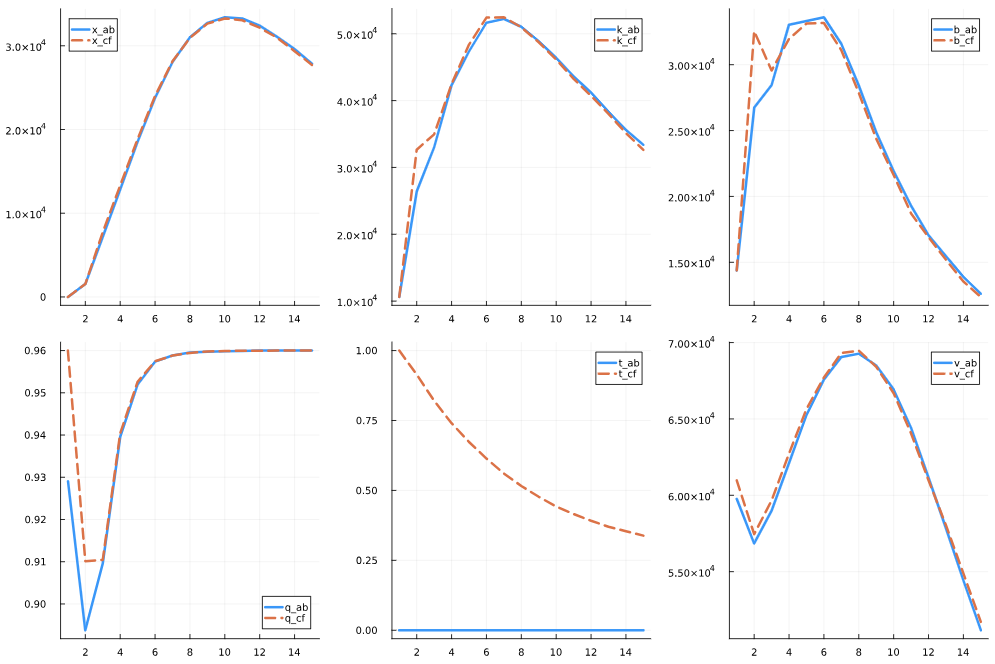
\includegraphics[width=1\textwidth]{C:/Users/szjud/OneDrive/Asztali gép/EBCs/CFL-git/Latex codes/Plots/dynsim.png}
    \caption{Firm lifecycle simulations} \label{chart:dynsim}
\end{figure}

\noindent Figure \ref{chart:DnQ} present a similar piece of evidence. It shows that average optimal policies across firms sizes. On the left panel, I take the 10-base logarithm of average debt. Similarly to the previous exercise, this result indicates that while optimal values of debt do not change for either calibrations the external finance premium is much larger when firms have no access to CF-based debt. 

\begin{figure}[H]  % [h] indicates placing the image here
    \centering
    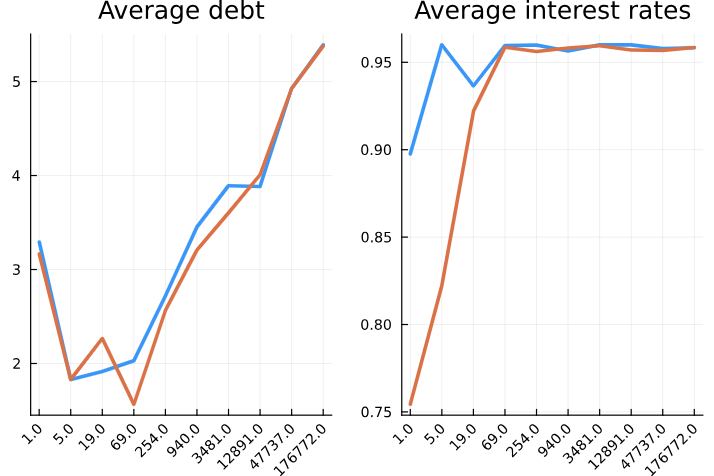
\includegraphics[width=0.9\textwidth]{C:/Users/szjud/OneDrive/Asztali gép/EBCs/CFL-git/Latex codes/Plots/DnQ.png}
    \caption{The log of debt and the inverse gross interest rate across firm sizes} \label{chart:DnQ}
\end{figure}

\noindent Gonzalez and Sy (2024) documents on a comprehensive dataset of Spanish firms that the average reliance on CF-based debt is U-shaped across firms sizes. Interestingly, the US firms covered in Compustat display a similar behavior.  Moreover, as shown in figure \ref{chart:Ushape}, the structural setup proposed here replicates this pattern (even without specifically targeting this result). However, the explanation proposed by Gonzalez and Sy (2024) is fundamentally different to what is suggested by my model. Their explanation rest on the following four assumptions: \textit{1)} firms face a variable cost of pledging collateral; \textit{2)} asset-backed loans have lower interest rates; \textit{3)} there are microeconomic cost of capital adjustment and \textit{4)} the pledgeability of earnings is such that earings-based constraints are less restrictive for small firms. In their model, assumption \textit{1-3} are necessary to match the right hand side of the U-shape and assumption \textit{4} matches the left hand side. \vspace{3mm} \\
In contrast, my model suggests that the optimal reliance on cash flow-based debt is determined by two factors: the relative value of continuation versus pledgeable assets and the probability of liquidation under financial distress. Firms on the left-hand side of the U-shape, typically productive entrants, with scarce pledgeable assets but high continuation values. This makes high reliance to on CF-based debt advantageous to them. On the right-hand side of the U-curve, large corporations face a near-zero probability of liquidation, which mitigates the risk of lending against future cash flows. This minimizes the downside of this type of debt, enabling these firms to heavily rely on CF-based debt.

\begin{figure}[H]  % [h] indicates placing the image here
    \centering
    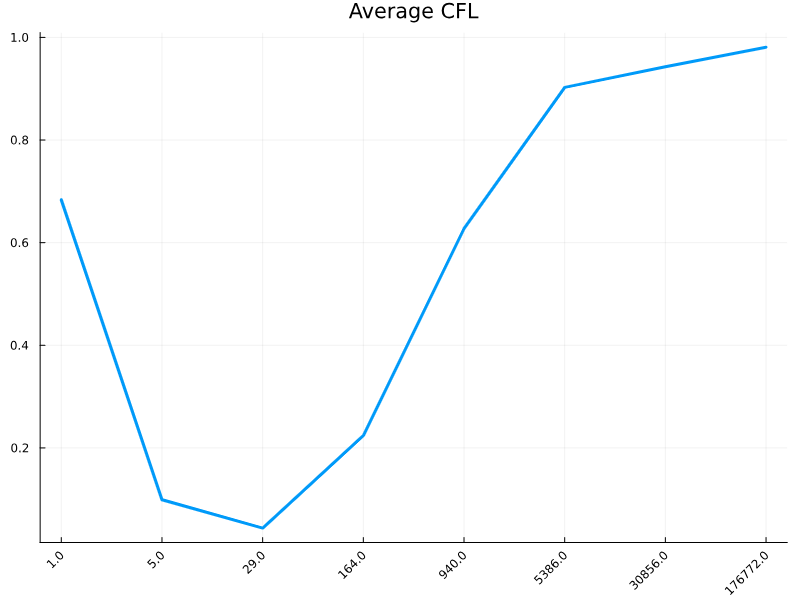
\includegraphics[width=0.65\textwidth]{C:/Users/szjud/OneDrive/Asztali gép/EBCs/CFL-git/Latex codes/Plots/Ushape.png}
    \caption{The U-shape: average reliance on CF-based debt across firm sizes} \label{chart:Ushape}
\end{figure}

\noindent Finally, consider the histogram of CF-reliances. One notable limitation of previous models is that they are unable to reproduce CF-reliance that is between zero and one. My model allows firms to choose any $\tau \in [0,1]$. This could be an nice innovation, but as figure \ref{chart:histog} shows, most firms still prefer to a CF-reliance relatively few firms choose CF-reliance between zero and one. \textit{I went out of my way to achieve this result, but I am not sure if it is worth it.}

\begin{figure}[H]  % [h] indicates placing the image here
    \centering
    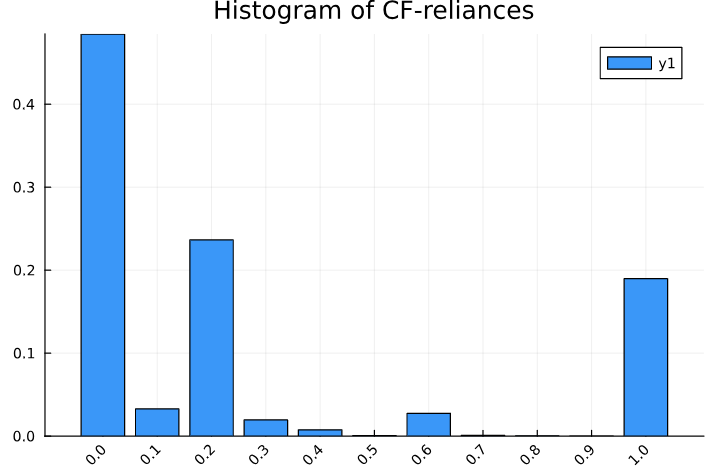
\includegraphics[width=0.8\textwidth]{C:/Users/szjud/OneDrive/Asztali gép/EBCs/CFL-git/Latex codes/Plots/histog.png}
    \caption{The histogram for CF-reliances} \label{chart:histog}
\end{figure}


\newpage

\appendix
\section{Model Solution \label{sec: qualitative analysis}}

In the structural model discussed above, optimal firm policies and the interest rate schedule offered by the lender are jointly determined. That is, lenders set interest rates based on firm policies, but firms choose these policies in light of the interest rate schedule offered to them. This presents a computational issue specific to this model setup. To address this, I adopt the following solution algorithm:\footnote{I similar algorithm is adopted by Corbae and D'Erasmo (2021).}
\begin{enumerate}
    \item Set $q^0 = 0$, the starting interest rate for all firm policies and calculate the value of the firm, $V_{cont}(k,b,\varepsilon)$, the optimal firm policies $k', b', \tau'$ as well as the exit and liquidation policies. 
    \item Calculate the following: the probability of default $P_D$, the probability of liquidation in default $\gamma$, the liquidation value; $\phi_A (1-\delta) k'$ and the reorganization value; $\phi_c V (x', \varepsilon')$ given $q^0$, for each state and firm policy pair
    \item Update interest rate associated with the state-action pair, taking into account the default and liquidation probability and lenders in-default payoffs. This gives  $q^1$. 
    \item Repeat $1-3$ until the optimal policies and interest rates do not change - that is, $ (k^{i},b^{i},\chi_d^{i},q^{i}, V^{i}) = (k^{i-1},b^{i-1},\chi_d^{i-1}, q^{i-1}, V^{i-1}) $.
\end{enumerate}
This algorithm is relatively robust, but it comes at a great computational cost. It usually takes around 30 to 50 iterations to converge, which implies the same number separate solutions of the firm optimization (step number 1) and updating the interests rate schedule (step number 2 and 3). To keep this computational demand manageable, I attempt keep the model as simple as possible in every other respect.

\section{Fixed Costs CF-based Lending \label{sec:fixed costs}}
In section \ref{sec:Default Resolution}, I adopt a highly stylized description of fixed costs: fixed costs of reorganization are imposed only on households which allows me to match the high liquidation probability associated with small corporations. In the interest of keeping the model simple, I do not impose a separate fixed costs on lenders. In practice however, this involves a lengthy negotiation between debtors, creditors, and courts, which imposes significant costs on every involved parties. Hence, when in-default payments are expected through reorganization, the lender must take into account the legal, personnel and time expenses of this process. \vspace{3mm} \\
However, maintaining a cash flow-based debt contract may impose significant costs on the lender even in the normal course of business. Asset-based contracts only require occasional audits of the borrower's assets. In contrast, cash flow-based contracts necessitate that the lender carries out its `due diligence' on an ongoing basis. The apparatus to maintain this monitoring activity may impose significant expenses on creditors.\footnote{This type of cost shares some similarities with the costly state verification first proposed by Towsend (1979).} More generally, such costs could be thought of as all additional expenses lenders face on a regular basis, when they deviate from standardized asset-based contracts.
\vspace{3mm} \\
In summary, evidence would also support for imposing additional fixed costs on creditors for lending against future cash flows. In fact, it would be possible to coin the central trade-off of the model in terms of these fixed cost. In this scenario, asset-based debt would provide the benefit of not having to monitor borrower performance and would offer a quick and cost-effective way of retrieve in default payments. Conversely, CF-based contracts would allow to potentially retrieve a share of the continuation value, but it would impose significant fixed costs on the lender. I do not include this mechanism in the model, as it would produce very similar results to the baseline setup. However, it is important to note that these fixed costs may influence lenders to favor one loan type over another.

\section{Bankruptcy Codes and Practices \label{sec:A1}}
\subsection{Key Principles \label{sec:key principles}}
In the following I highlight some of the key principles laid down in the US bankruptcy code. In this discussion, I highlight those that inform the structural model. \vspace{3mm} \\
\textit{a) The decision to reorganize or liquidate initially lies with the debtor, but lenders may be able enforce the conversion of the case.} Bankruptcy codes typically expect the debtor to first file for liquidation or reorganization - hence, the initial decision is in the hand of the debtor. Creditors may apply for the conversion of the case, but this is approved only under special circumstances. Overall, the influence of a single lender over the default resolution is limited. In the model, I assume that the liquidation decision is made by a third party - the household. However, when making the liquidation decision the household does not take into account the lender's payoffs. This reflects the fact that borrowers have more influence on the default resolution process. \vspace{3mm} \\
\textit{b) Reorganizations must comply with the `best-interest-of-creditors' test.} This rule states that no dissenting creditor should be worse off under the proposed reorganization plan than it would be under the liquidation of the debtor. I refer to this principle as a basis to assume that can consistently expect to recover at least the liquidation value of the firm, when the debt contract is asset-based. \vspace{3mm} \\
\textit{c) Special provisions to facilitate reorganization of SMEs}. Bankruptcy codes often attempt to alleviate the reorganization costs for small enterprises.\footnote{The EU directive allows member states to introduce special provisions to speed up and simplify the reorganization process for SMEs. The US bankruptcy code allow SMEs to file for a small business case (11 U.S.C. § 101(51C)) or under subchapter V of the Small Business Reorganization Act (SBRA), both of which are intended to streamline the reorganization process and reduce costs.} This is based on the recognition that these costs are often prohibitive for small corporations. In the model, I consider the effects of this policy by assuming that small firms only have to pay a fraction of the reorganization cost. However, it should be noted that despite of the special provisions in place, SMEs are still far more likely to choose liquidation. This could be interpreted as evidence that fixed costs of reorganization are still significant for small firms. 

\subsection{Common Themes of Bankruptcy Codes}
The US Bankruptcy Code is structured into chapters, each corresponding to a different type of relief for debtors in financial distress. In this paper, I focus on, chapter 7 deals with liquidations and chapter 11 regulates the reorganization process of US corporations. The European Union does not have a single bankruptcy code, but it has been working towards harmonizing insolvency proceedings across member states, based on the understanding that divergent insolvency laws create barriers across member states. As a result, the Harmonisation Directive\footnote{Directive (EU) 2019/1023 of the European Parliament and of the Council of 20 June 2019 on preventive restructuring frameworks, on discharge of debt and disqualifications, and on measures to increase the efficiency of procedures concerning restructuring, insolvency and discharge of debt.}  was published in June 2019, and member states are required to adopt the necessary legislative changes by July 2021 to comply with it. Although it does not completely standardize bankruptcy procedures, the directive outlines several principles that mirror the main features of chapter 7 and 11 of the US bankruptcy code. It represents a valuable piece of evidence for this discussion, as it collects the set of principles that legislators aim to institute in bankruptcy proceedings. \vspace{3mm} \\
Under both frameworks, the debtor is expected to file for insolvency – although creditors may petition the court to initiate bankruptcy proceedings against the debtor, this is not the norm. If the debtor decides to draft a reorganization plan, creditors may form committees and have their claims heard by courts. The European Union has a more debtor-friendly approach, meaning that creditors have less influence over the outcome of the proceedings, whereas the US system places more weight on the interest of the creditors. However, it is often the case that a debtor has numerous creditors, which limits the influence of any individual creditor over the specifics of the bankruptcy proceedings. 
\vspace{3mm} \\
Notably, both bankruptcy frameworks adhere to the `best interest of creditor test'. The EU Directive refers this as ‘best-interest-of-creditors’ test in OJ L 172/27, art. 49; whereas the US bankruptcy code establishes this principle in chapter 11 U.S. Code § 1129. Moreover, they also both provide special provision for small companies to reorganize at a smaller cost. The EU directive allows member states to introduce special provisions to speed up and simplify the reorganization process for SMEs. The US bankruptcy code allow SMEs to file for a small business case (11 U.S.C. § 101(51C)) or under subchapter V of the Small Business Reorganization Act (SBRA), both of which are intended to streamline the reorganization process and reduce costs.



\section{Data appendix \label{sec:A3}}
\subsection{Compustat and Capital IQ}
Compustat is a comprehensive, financial database maintained by S\&P Global. It offers standardized firm-level information on publicly traded companies compiled from financial statements, regulatory filings and other financial reports. I use the quarterly tables in Compustat North America and drop firms that are not headquartered in the US. Moreover, I exclude financial corporations (SIC code 6000 to 6799) and utility providers (SIC code 4900-4999). \vspace{3mm} \\
S\&P Capital IQ offers an extensive array of debt-level statistics. The two datasets can be connected via the unique firm a identifier (GVKEY), moreover Capital IQ covers most of the Compustat firms and yields consistent firm-level debt data after the aggregation of debt contracts. Although Capital IQ covers most major economies, I only focus on North American corporations, due to limitations introduced by Compustat.  \vspace{3mm} \\
Although both datasets provide high quality reports, reporting differences necessitate some manipulation of the data. Since monetary variables are often reported in the native currency, I bring all observations to USD. Moreover, Capital IQ reports data points in different units (units, thousands or millions). To be consistent to Compustat, I bring all observations to millions of units. It must also be ensured that each observation is uniquely identified by the combination of year, quarter, and debt ID. This may be violated for various reasons, for instance, debt facilities are often reported twice (once with the total accessible debt and once with the currently outstanding amount). Moreover, subsidiaries are also often included in the data. I exclude these to maintain observations at the highest consolidation level. \vspace{3mm} \\
In some instances, debt contracts go missing only to reappear a few quarters later. If this gap between observations is no more the 4 quarters, I use linear interpolation to fill up the data. These cases are relatively rare, they only amount to approximately 7\% of the total sample. To ensure the alignment of consistent observations, I aggregate debt-level data from CapitalIQ to the firm level and cross-reference it with the debt information reported by Compustat. I drop any observations where there is a disparity of more than 20\% between the two datasets. This discards around 8\% of the original sample. Tables \ref{tab:COMPS} and \ref{tab:CAPIQ} summarize Compustat and Capital IQ variables, including their original names and definitions in these datasets.

\begin{table}[htbp]    
\centering
\caption{Compustat variable definitions}
\label{tab:COMPS}
\renewcommand{\arraystretch}{1.5} % Increase the vertical spacing of rows
\resizebox{\textwidth}{!}{%
\begin{tabular}{lp{5cm}p{7cm}} 
\toprule
Variable & Compustat Definition & Description \\
\midrule
Total debt & dlcq+dlttq & Long-Term Debt + Debt in Current Liabilities \\
Leverage & (dlcq+dlttq)/atq & Total debt / Total Assets \\
Collateral & ppentq+invtq+rectq & Total Property, Plant and Equipment (net) + Receivables + Inventory \\
Pledgeability & (ppentq+invtq+rectq)/atq & Collateral / Total Assets \\
Interest coverage & oibdpq / xintq & Operating income before depreciation / Interest related expenses \\
Investment & capxq-sppeq & Capital expenditures - Sale of Property \\
Investment rate & (capxy - sppey) / l.ppegtq & Investment / Lag of Total Property, Plant and Equipment (gross) \\
Equity & atq-ltq & Total assets / Total liabilities \\
Net debt & dlcq+dltq-chq & Total debt - Cash Holdings \\
Liquidity & chq/atq & Cash Holdings / Total Assets \\
Assets & atq & Total Assets (book value) \\
Liabilities & ltq & Liabilities (book value) \\
Revenue & revtq & Total quarterly revenue \\
EBITDA & oibdpq & quarterly EBITDA measure \\
Employees & emp & Total number of employees (thousands) \\
Industry spec. & sic & SIC code \\
Credit rating & spcsrc & S\&P credit rating \\
Added value & revtq - cogsq & Total revenue - Input costs \\
Productivity & $\frac{revtq - cogsq}{ppegtq^{1/3} + emp^{2/3}}$ & Added value / Assets and Employees \\
Age & from Capital IQ & Current year - Year founded + 1 \\
\bottomrule
\end{tabular}
}
\end{table}

\newpage

\begin{table}[htbp]    

\centering
\caption{Capital IQ Variables}
\label{tab:CAPIQ}
\begin{tabular}{ll}
\toprule
Variable & Capital IQ \\
\midrule
Loan value & dataitemvalue \\
Decimal of the value & unittypeId \\
Currency of issuance & issuedCurrencyId \vspace{3mm} \\
\multicolumn{2}{l}{\textbf{Used for classification}} \\
Description of the contract & capitalstructuredescription \\
Type of the debt contract & capitalstructuresubtypeid \\
Debt description in text & descriptiontext \\
Secured dummy & securedtypeid \\
Seniority & leveltypeid \vspace{3mm} \\
\multicolumn{2}{l}{\textbf{Firm-level aggregated variables}} \\
Total debt value & Sum of all contracts value \\
AB value & Sum of all AB debt \\
CF value & Sum of all CF debt \\
CF share & CF value / Total debt \\
\bottomrule
\end{tabular}
\end{table}

\section{Additional Figures}

\noindent In line with the previous findings of Lian and Ma (2021) and Öztürk (2022), the total outstanding debt volume that can be classified as CF-based is relatively stable around 75\%. However, starting from 2019, this share drops significantly - from 79\% in 2018Q4 to 71\% 2019Q4 - and it does not fully recover until the end of the sample. It is not clear what causes this abrupt shift in aggregate CFL reliance. Unfortunately, I cannot compare with previous studies because they do not investigate this time period. One explanation could be the Covid-induced economic crisis. However, this leaves the initial drop. which happen before the pandemic had a substantial impact on North American economies unexplained. 

\begin{figure}[H]  % [h] indicates placing the image here
    \centering
    \caption{The share of cash flow-based debt to total debt} \label{chart:CFLshare}
    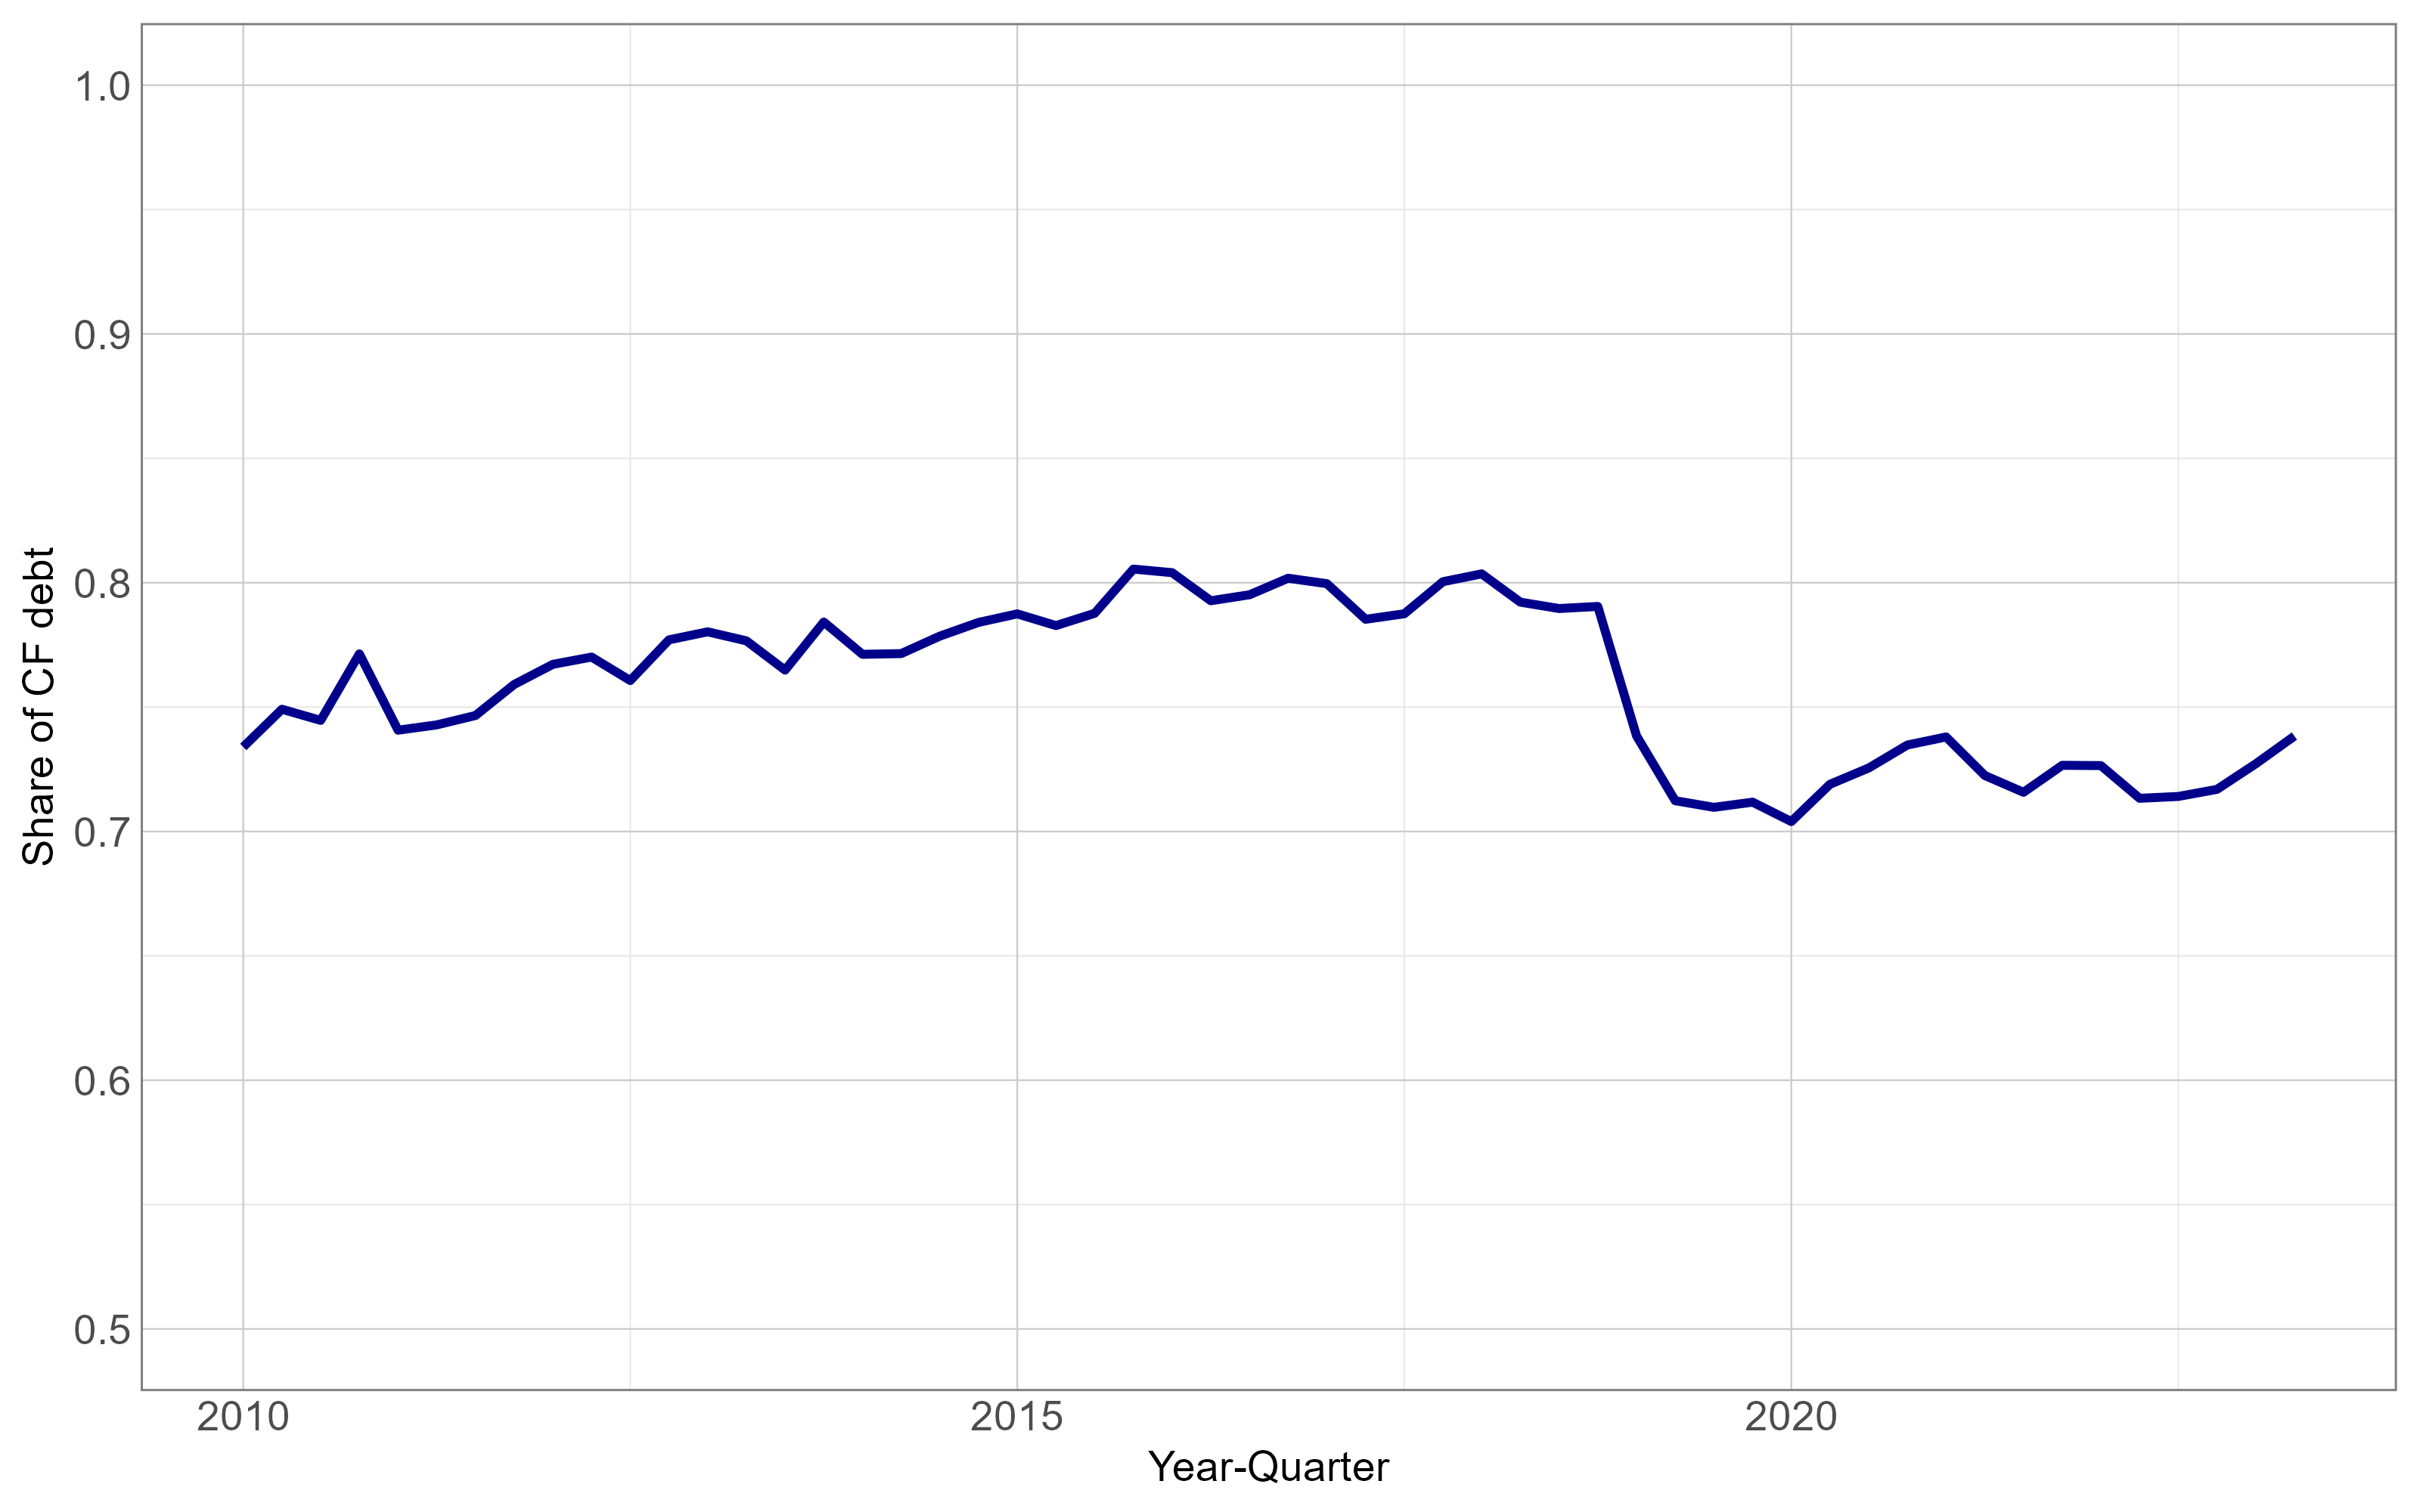
\includegraphics[width=0.7\textwidth]{C:/Users/szjud/OneDrive/Asztali gép/EBCs/CFL-git/Latex codes/Plots/CFshare.png} \\
     \small The share CFL debt to total debt, by volume between 2010Q1 and 2023Q3
\end{figure}

\noindent The figure below shows a stylized graph of the exit - default - continuation decisions of firms. 
\begin{figure}[H]  % [h] indicates placing the image here
    \centering
    \caption{The liquidation decision} \label{chart:DEC}
    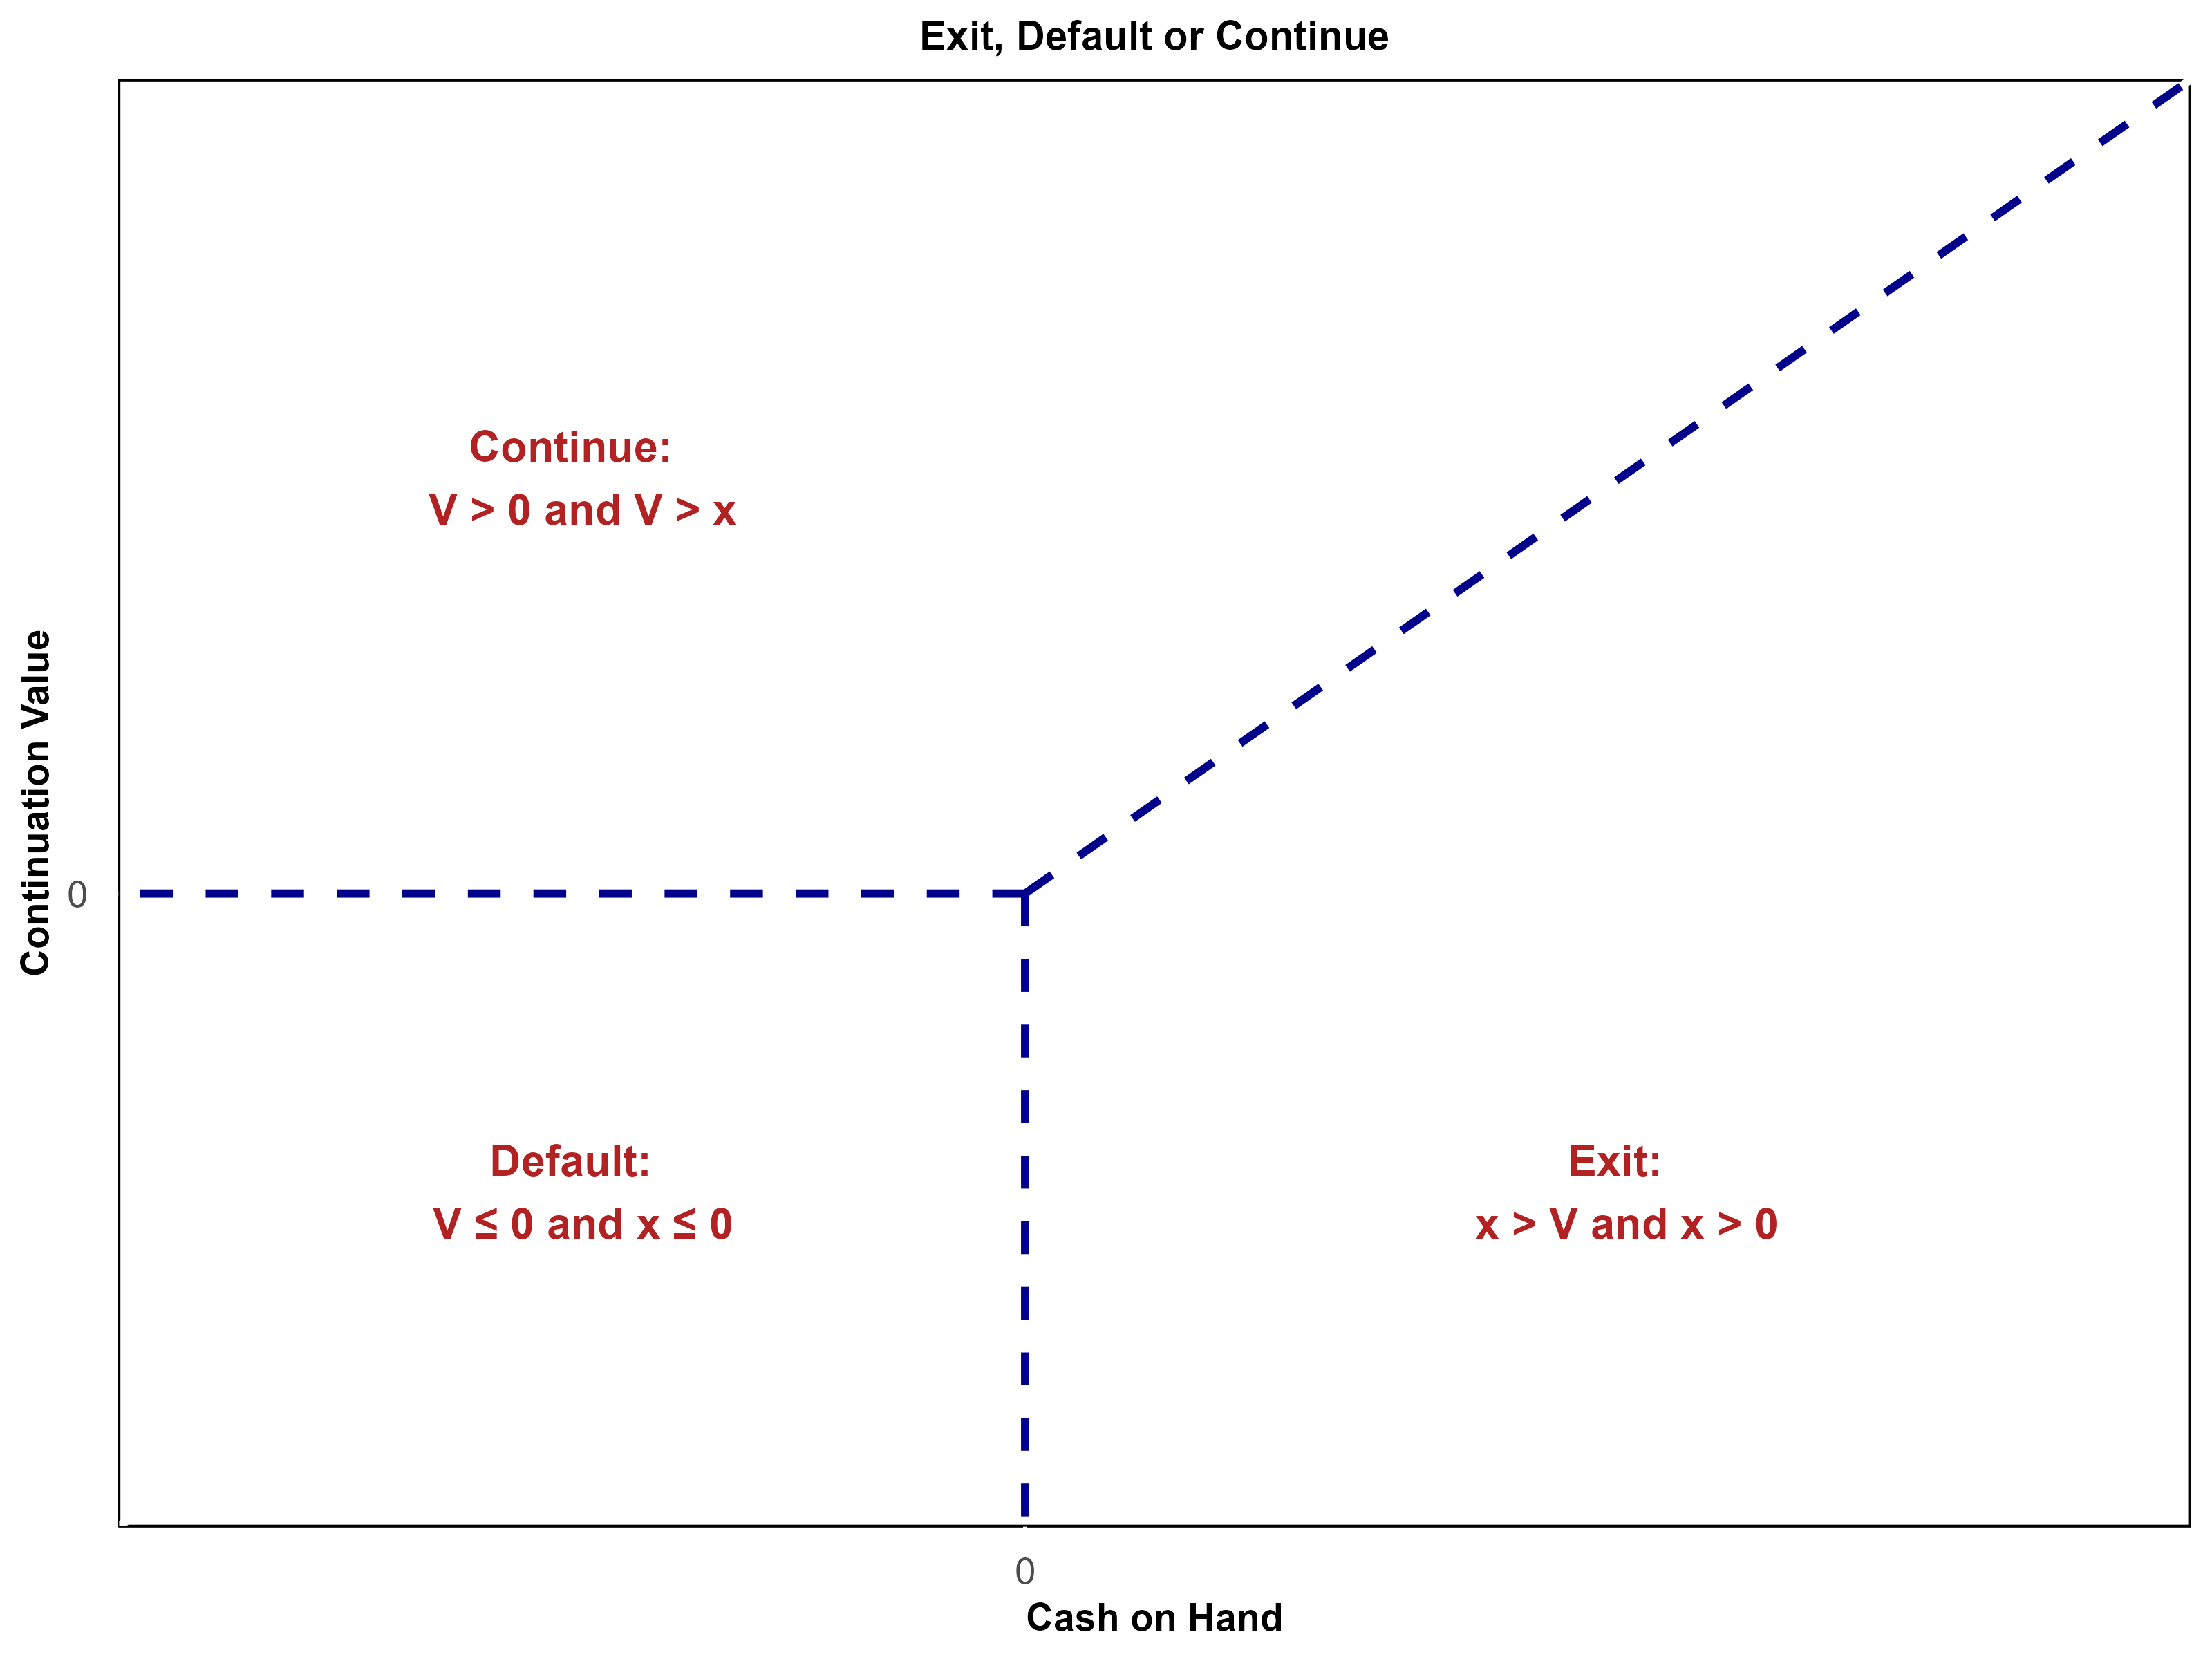
\includegraphics[width=0.7\textwidth]{C:/Users/szjud/OneDrive/Asztali gép/EBCs/CFL-git/Latex codes/Plots/dec.png}
\end{figure}

\end{document}